%\documentclass{article}
\documentclass[prl, longbibliography]{revtex4-2}
\usepackage{graphicx}
\usepackage{makecell}
\usepackage{amsmath}
\usepackage{mathtools}

\begin{document}

\title{Mark's Notes on Molecular Potential Calculations}
\author{Mark O. Brown}

\begin{abstract}
A discussion of the calculation of molecular potentials incorporating Dipole-Dipole interactions, fine structure, molecule rotation, and eventually fine structure. These calculations mostly come from old photoassociation experiments and are surprisingly inaccessible to the lowly atomic physicist. The goal of this document is therefore a very pedagogical description of the calculations, aimed at those who have no experience with molecular physics and only a passing familiarity with hydrogen-like atoms as seen in an introductory quantum mechanics class. 
\end{abstract}

\maketitle

\section{Introduction}
Most of the work in our lab is with individual Rubidium 87 atoms, or of many weakly-interacting Rubidium 87 atoms in their electronic ground-states. 
In this case, atom-atom interactions can be approximated as S-wave collisions that are parameterized by a single constant - the scattering length. 
For Rubidium-87 this is $a_{sc}\approx97 a_0$ where $a_0$ is the bohr radius, although the value varies by $~1\%$ depending on the hyperfine states of the interacting atoms\cite{egorov_precision_2013}. 

However, there is a major case where this simplified picture does not apply, which is in the case of loading atoms into the tweezer in the first place using light-assisted collisions. In this case, atoms are excited by the loading light into a molecular potential which causes a great amount of heating of pairs of atoms, generally causing pairs of atoms to be lost from the tweezer. The dynamics of the loading procedure are presumably then very dependent on the details of the molecular structure of the atoms. We became especially interested in this material upon discovering our Grey-Molasses based loading technique, and subsequently began to study these structures in greater detail in order to illucidate the exact mechanisms of the loading technique and hopefully to be able to predict and improve loading rates. 

While Rubidium 87 is a simple alkali-earth atom, calculating the molecular potentials experienced by two such atoms is technically rather challenging. 
Despite the prevailance of Rubidium 87, these calculations are not generally known in the region of interest for the experiment. 
The relevant energy scale for the experiment is about 20MHz, since this is the trap depth. The molecular interactions reach this scale at on the order of ~100nm for S\&P atoms. 
Most of the work done on the calculation of molecular potentials comes from old photoassociation spectroscopy work, however the typical energy scales of interest here are many orders of magnitude larger than those of interest to us. However, several photoassociation review articles\cite{jones_ultracold_2006, weiner_experiments_1999} are still especially useful here.
As a result, most of the calculations in the field don't go so far as to include, e.g., the hyperfine splitting.

Several books are also useful references, especially for some of the theory regarding the symmetries in molecules \cite{lefebvre-brion_perturbations_1986}. 

\section{Atomic Wavefunctions}

The baseline for all the molecular calculations here are the hydrogen atom states. And so I review the notation relevant to the hydrogen atom here. Hydrogen atom wavefunctions come from solving the following equation:
\begin{equation}
E|\psi\rangle = \bigg(-\frac{\hbar^2}{2m}\nabla^2 - \frac{e^2}{4\pi\epsilon_0}\frac{1}{r}\bigg)|\psi\rangle
\end{equation}
As the equation is spherically symmetric, the above equation is separable into an angular equation and a radial equation. 
Furthermore the equations can be parameterized in terms of the angular momentum operator $\hat{L}=\hat{r}\times\hat{p}$. 
The solutions of the angular equation are the spherical harmonics, typically identified with quantum numbers $\ell$ and $m_\ell$, related to the angular momentum operator by $\hat{L}^2|\ell,m_\ell\rangle = \hbar^2 \ell (\ell+1)|\ell,m_\ell\rangle$ and $\hat{L}_z|\ell,m_\ell\rangle = \hbar m_\ell|\ell,m_\ell\rangle$.  
The solutions of the radial equation are wavefunctions typically identified with quantum numbers $n$ and $\ell$. 
Therefore, the solutions to the hydrogen atom problem can be identified by three quantum numbers, and are therefore typically represented by the following kets: $|\psi\rangle=|n\ell m_\ell\rangle$.
Further, in relativistic treatments one finds that particles have spin, and so the total wavefunction should include these spin states. 
The electron spin is typically given quantum numbers $s$ and $m_s$, and the nucleus is typically given quantum numbers $i$ and $m_i$.
Therefore, to first order the full state of the atom can be given by the following kets: $|n;\ell m_\ell; s m_s; i m_i\rangle$. 

However, spins have magnetic moments which create magnetic fields, and so all of the spins interact with each other. 
The fine structure correction thusly includes a term $H_{fs}=A \hat{L}\cdot\hat{S}$. While $\hat{L}^2$ and $\hat{S}^2$ commute with $H_{fs}$, $\hat{L}_z$ and $\hat{S}_z$. It is then typical to define $\hat{J}=\hat{L}+\hat{S}$ and then find that both $\hat{J}$ and $\hat{J}_z$ commute with $H_{fs}$. 
As such, we replace the quantum numbers $|\ell m_\ell; s m_s\rangle\rightarrow|j m_j \ell s\rangle$ where the $\ell$ and $s$ are oftentimes implicit.
To change bases one then uses the equation:
\begin{equation}
|j m_j \ell s\rangle = \sum_{m_s, m_\ell} \langle \ell m_\ell s m_s | j m_j \ell s\rangle| j m_j \ell s\rangle = \sum_{m_s, m_\ell} C_{\ell m_\ell s m_s}^{j m_j}| j m_j \ell s\rangle
\end{equation}
Where the constants $C_{\ell m_\ell s m_s}^{j m_j}=\langle \ell m_\ell s m_s | j m_j \ell s\rangle$ are the Clebsch-Gordon coefficients. Similarly, there is a much smaller but still significant hyperfine interaction of the form $B \hat{J}\cdot\hat{I}$. It is typical to define $\hat{F} = \hat{J}+\hat{I}$ and similar analysis follows, leading to the following basis for the hydrogen atom:
\begin{equation}
|\psi\rangle = |n F m_F; ij\ell s\rangle
\end{equation}
where again, depending on the context, the values of $i,j,\ell,$ and $s$ are often obvious and therefore dropped from the ket. The values for the fine structure and hyperfine structure constants $A$ and $B$ are typically determined experimentally. 

\section{Notation}

Now, we must introduce a much more complicated notation for describing the molecular states. In the single-atom case we had 5 important angular momenta to consider: $\hat{L}, \hat{S}, \hat{I}, \hat{J},$ and $\hat{F}$. Now, we have at least all of these angular momenta for both atoms, plus the rotational angular momenta, and many more combinations thereof. Moreover, the notation in the molecular spectroscopy literature is moderately pathological, even given this, ditching common patterns found in atomic physics. While right now we only have need for $\hat{L}=\hat{L}_a+\hat{L}_b$, I report all the angular momenta in table 1. 

\begin{center}
\begin{tabular}{ ||c|c|c|c|c|c||  }
 \hline
 Description & \makecell{Angular \\Momentum \\Operator $\hat{Z}$} & \makecell{$\hat{Z}^2$ Eigenvalues \\($\hbar^2 z(z+1)$)} & \makecell{Body-Fixed\\ $\hat{Z}_z$ Eigenvalues \\($\hbar m_z$)} &\makecell{Space-Fixed\\ $\hat{Z}_z$ Eigenvalues \\($\hbar m_z$)} & \makecell{Alternative \\Representations}\\
 \hline
 \hline
 Single Electron Orbital A.M. & $\hat{L}_\alpha$ & $L_\alpha$ & $\Lambda_\alpha$ & $m_{L_\alpha} $ & None \\
 \hline
 Net Electron Orbital A.M. & $\hat{L}$ & $l$ & $\Lambda=\Lambda_a+\Lambda_b$ &$m_L $ & $\hat{L}=\hat{L}_a + \hat{L}_b$ \\
 \hline
 Single Electron Spin & $\hat{S}_\alpha$ & $S_\alpha$ & $\Sigma_\alpha$ &$m_{S_\alpha} $ & None \\
 \hline
 Net Electron Spin & $\hat{S}$ & $S$ & $\Sigma=\Sigma_a+\Sigma_b$ &$m_S $ &  $\hat{S}=\hat{S}_a + \hat{S}_b$ \\
 \hline
 Single Electron Net A.M. & $\hat{j}_\alpha$ & $j_\alpha$ & $\Omega_\alpha=\Lambda_a+\Sigma_a$ &$m_{j_\alpha} $ &  $j_\alpha = L_\alpha+S_\alpha$ \\
 \hline
 Net Electron A.M. & $\hat{j}$ & $j$ & $\Omega=\Lambda+\Sigma$ &$m_j $  & $\hat{j} = \hat{L}+\hat{S}$ \\
 \hline
 Net A.M. Except Nuclear Spin & $\hat{J}$ & $J$ & Also $\Omega$ &$m_J $  & $\hat{J}=\hat{L}+\hat{S}+\hat{N}$ \\
 \hline
 Nuclear Rotational A.M. & $\hat{N}$ & $\ell$ & $0$ (Always) & $\mu$ &  $\hat{N} = \hat{J} - \hat{L} - \hat{S}$ \\
 \hline
 Single Nuclear Spin & $\hat{i}_\alpha$ & $i_\alpha$ & $\iota_{\alpha}$ &$m_i $ &  None \\
 \hline
 Net Nuclear Spin & $\hat{I}$ & $I$ & $\iota=\iota_a+\iota_b$ &$m_I $ &  $\hat{I}=\hat{i}_a+\hat{i}_b$ \\
 \hline
 \makecell{Net Mechanical A.M.\\(Relevant in Hund's cases (b) and (d))} & $\hat{K}$ & $K$ & (Rare)$\kappa$? &$m_K $ &  $\hat{K}=\hat{L}+\hat{N}$ \\
 \hline
  Single Atom Net A.M. & $\hat{f}_\alpha$ & $f_\alpha$ & $\phi_\alpha=\Omega_\alpha+\iota_{\alpha}$ &  $m_{f_\alpha} $& $\hat{f}_\alpha=\hat{j}_\alpha+\hat{i}_\alpha$ \\
 \hline
   Total Non-Rotatoinal A.M. & $\hat{f}$ & $f$ & $\phi=\Omega+\iota$ &  $m_f $& $\hat{f}=\hat{j}+\hat{i}$ \\
 \hline
  Total A.M. & $\hat{F}$ & $F$ & Also $\phi$ &$m_F $ &  $\hat{F}=\hat{J}+\hat{I}$ \\
 \hline 
\end{tabular}
\end{center}

Notice in particular that this notation primarily uses greek letters as the projection eigenvalues. Oftentimes in the notation, only the magnitude of the projection is important, not it's sign. Note as well that the symbols for the projections of various on the angular momentum ($\Lambda, \Sigma, \Omega$) are not to be confused with the labels of different values of $\Lambda$ ($\Lambda=0$ gets labeled $\Sigma$, $\Lambda=1$ gets labeled $\Pi$, etc.). Very confusing. 

% %%%%%%%%%%%%%%%%%%%%%%%%%%%%%%%%%%%%%%%%%%%%%%%%%%%%%%%%%%%%
% %%%%%%%%%%%%%%%%%%%%%%%%%%%%%%%%%%%%%%%%%%%%%%%%%%%%%%%%%%%%
\section{Molecular Electronic Structure (Bohr-OppenHeimer Potentials)}
% %%%%%%%%%%%%%%%%%%%%%%%%%%%%%%%%%%%%%%%%%%%%%%%%%%%%%%%%%%%%
% %%%%%%%%%%%%%%%%%%%%%%%%%%%%%%%%%%%%%%%%%%%%%%%%%%%%%%%%%%%%

[Description of approximation here needs work] In the center of mass frame, the general homonuclear molecule problem can be stated as solving the following equation:
$$
E|\psi\rangle = -\frac{\hbar^2}{2m}(\nabla_a^2+\nabla_b^2 +\nabla_{R}^2) + \frac{e^2}{4\pi\epsilon_0} \Big(-\frac{1}{r_a} -\frac{1}{r_b} + \frac{1}{R} + \frac{1}{|\vec{r}_b-\vec{r}_a|}\Big)
$$

where $R$ is the internuclear distance. The "Adiabatic" Bohr-Oppenheimer (BO) approximation neglects the nuclear kinetic energy term since the nuclei move much slower than the much lighter electroncs for the same energy. 

In the atomic physics case, the potential was spherically symmetric, leading to having the nice Spherical harmonics as solutions to the angular part of the equation. Unfortunately, our potential is no longer spherically symmetric, but rather cylindrically symmetric about the internuclear axis ($\vec{R}$ points along this axis). For homonuclear molecules, it is also symmetric about a plane perpendicular to this axis sitting between the two nuclei. This cylindrical symmetry picks a natural axis for the projection of our angular momentum. Since I don't deal with external fields or polyatomic molecules at all in these notes, for the rest of the notes the projections of any angular momentum will always be along the internuclear axis.

This BO analysis is evidentally dealing with the interaction of the electrons with the nuclei themselves, which is the largest interaction in the atom. As such, the mangitudes of these potentials are on the order of the energy spacing between different angular momentum quantum numbers, so e.g. on the order of the D1 and D2 lines for alkali earths, or hundreds of THz. As well, the length scale at which these calculations are important is the length at which the overlap of the atomic electron wavefunctions about the two nuclei is significant, or typically $< 1nm$.

The symmetry-breaking molecular potential will generally mix states of different $n$ and $L$ (atomic notation), but not different $\Lambda$ (the projection of L along the internuclear axis) (e.g. it will mix $|nLm_L\rangle=|4,1,1\rangle$ with $|5,3,1\rangle$ but not $|4,1,1\rangle$ with $|4,1,0\rangle$. 
As a result, $n$ and $L$ are not good quantum numbers when the molecular interaction is significant, but $\Lambda$ is still a good quantum number. 
It is worth noting while $n$ and $L$ are not good quantum numbers in the sense that states in the BO potentials do not have well-defined values of them and that the hamiltonian does not conserve them, states are often still labeled by the values of these quantum numbers which a given state is connected to in the long-distance limit.
The potential does not interact with the spin of the electrons, therefore the total spin of the molecule $S$ is a second good quantum number. Furthermore, different spin states (singlet vs triplet) will have different energies due to the impact the spin state has on the symmetrization of the rest of the wavefunction.

Thirdly, because of the symmetry of homonuclear molecules about the plane bisecting the molecule, molecular states are eigenstates of operator inverting the z coordinate. The number in abstract is call $\sigma$ (note the lack of subscript differing it from the single-atom spin projection $\sigma_{a/b}$) Symmetric eigenstates are labeled $g$ for gerade" eigenstates, and antisymmetric eigenstates are labeled $u$ for "ungerade".

Lastly, states can also be eigenstates of the operator that flips the wavefunction about a plane \emph{containing} the internuclear axis. These states get labeled with a + or - depending on their parity, although there is an amiguity as to which plane to use for the flipping and therefore an ambiguity in which gets assigne + vs -\cite{lefebvre-brion_perturbations_1986}. However these are somewhat redundant in some cases since symmetrization considerations fixes their value, and the BO potential does not split them energetically. They will be split later by the fine-structure interactions. Therefore the $Pi$ states do not have good such numbers while $\Lambda=0$ are all + states. 

A good way to understand these symmetries and the relationships between them is by thinking in terms of the solutions to the $H_2^+$ ion. To first order, the electronic wavefunction will be a sum of the hydrogen atom solutions $|n,L,m_L\rangle$ centered around the two nuclei. For sample, one can have an even sum $|E\rangle=|n,L,m_L\rangle_R + |n,L,m_L\rangle_L$ and an odd sum: $|O\rangle=|n,L,m_L\rangle_R - |n,L,m_L\rangle_L$ which are even and odd respectively under the spatial inversion operator for a single electron. Then, to first order, (and keeping an eye on the incoming symmetrization requirements) the possible molecular states will be $|\psi\rangle=|EE\rangle, |OO\rangle,|EO\rangle+|OE\rangle,\text{ and } |EO\rangle-|OE\rangle$. The first two will be even under the inversion operator, and the second two will odd under the inversion operator, and hence the first two are gerade states and the second two are ungerade states. Furthermore, one can easily see that the first three states are symmetric under exchange of the particles, and the last is antisymmetric. Therefore, in order for the total electron wavefunction to by antisymmetric, the first three must be paired with a spin-singlet state, and the last must be paired with a spin triplet state. 

I need to consider the excitation. I can have an excited state with an even or odd spatial distribution. So I can have $|E'\rangle$ or $|O'\rangle$. So my two particle excited state can be:
$$
|O'O\rangle+|OO'\rangle, |E'E\rangle+|EE'\rangle,  |E'E\rangle-|EE'\rangle,|O'O\rangle-|OO'\rangle, |E'O\rangle+|OE'\rangle, \text{ and } |E'O\rangle-|OE'\rangle
$$
which are gerade and symmetric, gerade and antisymmetric, ungerade and symmetric, and ungerade and antisymmetric respectively. 


the solutions to the molecule without electron-electron interactions, as this is a common application of the variational principle in elementary quantum mechanics. If you assume that the solutions of a single electron are sums of the solutions to the individual atoms, then for either S or P atoms, you can quickly see solutions of the form $|\psi\rangle_{p/m}=|S\rangle _a \pm |S\rangle _b$. The + (-) state would be symmetric (antisymettric) with respect to reflection across a plane bisecting the molecule. Then, one can reasonably expect that the two particles will have a similar symmetry, and that you might have two particle states of the form $|\psi_+\psi_+\rangle,|\psi_-\psi_-\rangle, |\psi_+\psi_-\rangle, $ and $|\psi_-\psi_+\rangle$. The first two states would then be states of gerade (i.e. positive) parity, and the latter two states would be of ungerade parity. Now, it is more obvious how this parity interacts with the particle exchange parity. 

With these three main good quantum numbers, BO eigenstates typically get labeled by the following symbols: $^{2S+1}\Lambda_{g/u}$.
They can also be labeled in ket form with a more full set of quantum numbers $|L\Lambda\sigma S\Sigma\rangle$, or to be complete $|L\Lambda L_a L_b \sigma; S\Sigma S_a S_b\rangle$. 
For example, for alkali atoms the ground $S+S$ states split into only two states: $^3\Sigma^+_g$ and $^1\Sigma^+_u$. 
In fact, it is a common excersize to do a simple BO calculation for the H2 atom. It is much more complicated to do excited state calculations as the excited $S+P$ states split into $^3\Sigma^+_g$, $^3\Sigma^+_u$, $^1\Sigma^+_g$, $^1\Sigma^+_u$, $^3\Pi_g$, $^3\Pi_u$, $^1\Pi_g$, and $^1\Pi_u$. For more on these calculations, see e.g. \cite{magnier_potential_1993}. 

% %%%%%%%%%%%%%%%%%%%%%%%%%%%%%%%%%%%%%%%%%%%%%%%%%%%%%%%%%%%%
% %%%%%%%%%%%%%%%%%%%%%%%%%%%%%%%%%%%%%%%%%%%%%%%%%%%%%%%%%%%%
\section{Molecular Fine Structure (Movre-Pischler Potentials)}
% %%%%%%%%%%%%%%%%%%%%%%%%%%%%%%%%%%%%%%%%%%%%%%%%%%%%%%%%%%%%
% %%%%%%%%%%%%%%%%%%%%%%%%%%%%%%%%%%%%%%%%%%%%%%%%%%%%%%%%%%%%

\cite{bergeman_predissociations_2002} is a good reference for this calculation. The atomic fine-structure correction for atom $a$ is given by $A \hat{L}_a\cdot\hat{S}_a$ where $A$ is an experimentally determined constant. This energy scale becomes important as the BO energies become small at length scales where the electron overlap becomes small. So one might think that one should include internuclear coupling terms such as $\hat{L}_a\cdot\hat{L}_b$, however terms like this would only be significant where wavefunction overap is signficant, where the BO interactions overwhelmingly dominate. Therefore, here we consider the hamiltonian describing the system to be:
\begin{align}
H = H_{\text{BO,LO}} + H_{hf} \\
H_{hf}=A(\hat{L}_a\cdot\hat{S}_a+\hat{L}_b\cdot\hat{S}_b)
\end{align}

where $H_{\text{BO,LO}}$ represents the leading order contributions from the BO interactions. 
So generally the fine-structure interaction will result in a spatially varying mixing of the BO states, with the mixing becoming stronger and eventually becoming the normal single-atom mixed states in the long distance limit and being relatively weaker at short distances where the diagonal terms from the BO interactions dominate.
Generally the leading order contributions are some of the following: The dipole-dipole interaction, which goes as $C_3/R^3$, the qudrupole interaction which goes as $C_5/R^5$, and the van-der-walls interaction which goes as $C_6/R^6$. 
In general these constants and those higher order corrections have been measured or calculated (especially for common atoms like alkalis) and can be looked up (for example, \cite{marinescu_dispersion_1995} is a great reference here).

So, the key step in the calculation is the calculation of all $H_{BO,LO}$ matrix elements and all $H_{fs}$ matrix elements. So, lets begin with $H_{BO,LO}$. In many cases, there is no dipole-dipole interaction between the two atoms becaues neither the S nor the P atomic state has a permanent dipole, and so the leading order term is going to be the induced $~1/R^6$ van-der-wals interaction. However, for the S+P potentials in homonuclear molecules, due to symmetrization requirements each valence electron must be considered to be in a superposition of S and P, and in fact does have a permanent dipole moment. 

The dipole interaction is
\begin{equation}
V_{dd} = \frac{1}{4\pi\epsilon_0}\frac{\vec{d}_a\cdot\vec{d}_b - 3d_{az}d_{bz}}{R^3}=-p\frac{3\Lambda^2-L(L+1)}{R^3} C_3
\end{equation}

Where a citation is needed for the latter equality. These elements are then trivial to calculate for each BO state since $\Lambda$ and $L$ are both good quantum numbers. More complicated is the fine-structure interaction. The fine-structure interaction has eigenvalues
\begin{equation}
A(\hat{L_a}\cdot\hat{S_a})|J_a m_{J_a} L_a S_a\rangle = A\Big(J_a(J_a+1)-L_a(L_a+1)-S_a(S_a+1)\Big)|J_a m_{J_a} L_a S_a\rangle
\end{equation}
So to calculate the fine-structure interaction matrix elements, one must convert each two-atom BO state to the appropriate sum of single-atom fine-structure states to calcualte each element. This is not hard, each part of the BO state is simply given by a sum of angular momenta and so we are simply going to get a bunch of clebsch gordon coefficients. We have 
\begin{equation}
|L\Lambda L_a L_b\rangle=\sum_{\Lambda_a, \Lambda_b}\langle L_a \Lambda_a L_b \Lambda_b|L\Lambda L_a L_b\rangle\times|L_a \Lambda_a L_b \Lambda_b\rangle =\sum_{\Lambda_a \Lambda_b} C_{L_a \Lambda_a L_b \Lambda_b}^{L \Lambda} |L_a \Lambda_a L_b \Lambda_b\rangle
\end{equation}

Where $C_{L_a \Lambda_a L_b \Lambda_b}^{L \Lambda}$ are the Clebsch Gordon coefficients. However, the atom must be symmetrized, so espeically for the S+P case we must consider the appropriate symmetrization:
\begin{equation}
|L \Lambda \sigma\rangle \propto |L\Lambda L_a L_b\rangle + p |L\Lambda L_b L_a\rangle
\end{equation}
where p should be chosen to make the \emph{entire} wavefunction of the two electrons antisymmetric with respect to particle exchange. In the case that $L_a=L_b$ or for heteronuclear molecules, we can take $p=0$.  The other parts of the wavefunction that factor into this are the spin part and the spatial part, so we can therefor relate $p$ to the total spin and spatial quantum number of the state: 
\begin{equation}
p = (-1)^{S+\sigma}
\end{equation}
where $\sigma=0$ for gerade ("g") states and $\sigma=1$ for ungerade ("u") states.

The Spin is simpler since there's no additional symmetrization considerations:
\begin{equation}
|S \Sigma\rangle = \sum_{\Sigma_a \Sigma_b} C_{S_a \Sigma_a S_b \Sigma_b}^{S \Sigma} |S_a \Sigma_a S_b \Sigma_b\rangle
\end{equation}

Therefore, the total state is given by
\begin{equation}
|L\Lambda L_a L_b \sigma; S\Sigma S_a S_b\rangle = \sum_{\Lambda_a\Lambda_b\Sigma_a\Sigma_b} C_{L_a \Lambda_a L_b \Lambda_b}^{L \Lambda}C_{S_a \Sigma_a S_b \Sigma_b}^{S \Sigma}\big( |L_a\Lambda_a S_a \Sigma_a\rangle|L_b\Lambda_b S_b \Sigma_b\rangle + (-1)^{S+\sigma}|L_b\Lambda_b S_a \Sigma_a\rangle|L_a\Lambda_a S_b \Sigma_b\rangle \big)
\end{equation} 

From here it's straitforward if tedious to calculate the fine-structure matrix elements. I set up some code to do this automatically, but this is rather difficult to manage as well as it's not very natural to convert the angular momentum bases to column vectors. But it has been done.

One can be more specious though by looking at the symmetries of the fine-structure operators. Similar to L, j won't be a good quantum number, but the projection of j on the internuclear axis $\Omega$ will be. The fine structure operator won't mix states of different $\Omega$, different $\pm$, or different $g/u$ quantum numbers. Thus the total matrix will be block-diagonal in these states. As such, these states are typically labeled by symbols of the form $\Omega^{\pm}_{g/u}$ where $\Omega$ is half-integer.  I list the resulting sub-matrices below. 

\begin{equation}
\begin{gathered}
0^{-}_{g}:
\begin{bmatrix}
\frac{C_3}{R^3}-\frac{2\Delta}{3} & \frac{\sqrt{2}\Delta}{3}\\
\frac{\sqrt{2}\Delta}{3}&-\frac{2C_3}{R^3}-\frac{\Delta}{3}
\end{bmatrix}, \ 
0^{+}_{g}:
\begin{bmatrix}
\frac{C_3}{R^3}-\frac{2\Delta}{3} & \frac{\sqrt{2}\Delta}{3}\\
\frac{\sqrt{2}\Delta}{3}&\frac{2C_3}{R^3}-\frac{\Delta}{3}
\end{bmatrix},  \ 
0^{-}_{u}:
\begin{bmatrix}
-\frac{C_3}{R^3}-\frac{2\Delta}{3} & -\frac{\sqrt{2}\Delta}{3}\\
-\frac{\sqrt{2}\Delta}{3}&-\frac{2C_3}{R^3}-\frac{\Delta}{3}
\end{bmatrix},  \ 
0^{+}_{u}:
\begin{bmatrix}
-\frac{C_3}{R^3}-\frac{2\Delta}{3} & \frac{\sqrt{2}\Delta}{3}\\
\frac{\sqrt{2}\Delta}{3}&-\frac{2C_3}{R^3}-\frac{\Delta}{3}
\end{bmatrix} \\
1_{g}:
\begin{bmatrix}
\frac{C_3}{R^3}-\frac{\Delta}{3} & -\frac{\Delta}{3}&\frac{\Delta}{3}\\
-\frac{\Delta}{3}&-\frac{C_3}{R^3}-\frac{\Delta}{3}&\frac{\Delta}{3}\\
\frac{\Delta}{3}&\frac{\Delta}{3}&-\frac{2C_3}{R^3}-\frac{\Delta}{3}
\end{bmatrix}, \quad
1_{u}:
\begin{bmatrix}
-\frac{C_3}{R^3}-\frac{\Delta}{3} & -\frac{\Delta}{3}&\frac{\Delta}{3}\\
-\frac{\Delta}{3}&\frac{C_3}{R^3}-\frac{\Delta}{3}&\frac{\Delta}{3}\\
\frac{\Delta}{3}&\frac{\Delta}{3}&\frac{2C_3}{R^3}-\frac{\Delta}{3}
\end{bmatrix} \\
2_{g}:
\begin{bmatrix}
\frac{C_3}{R^3}
\end{bmatrix}, \quad
2_{u}:
\begin{bmatrix}
-\frac{C_3}{R^3}
\end{bmatrix}
\end{gathered}
\end{equation}

Diagonalizing all of these matrices realizes at every position $R$ yields the curves in figure 1.   
\begin{figure}
  \centering
    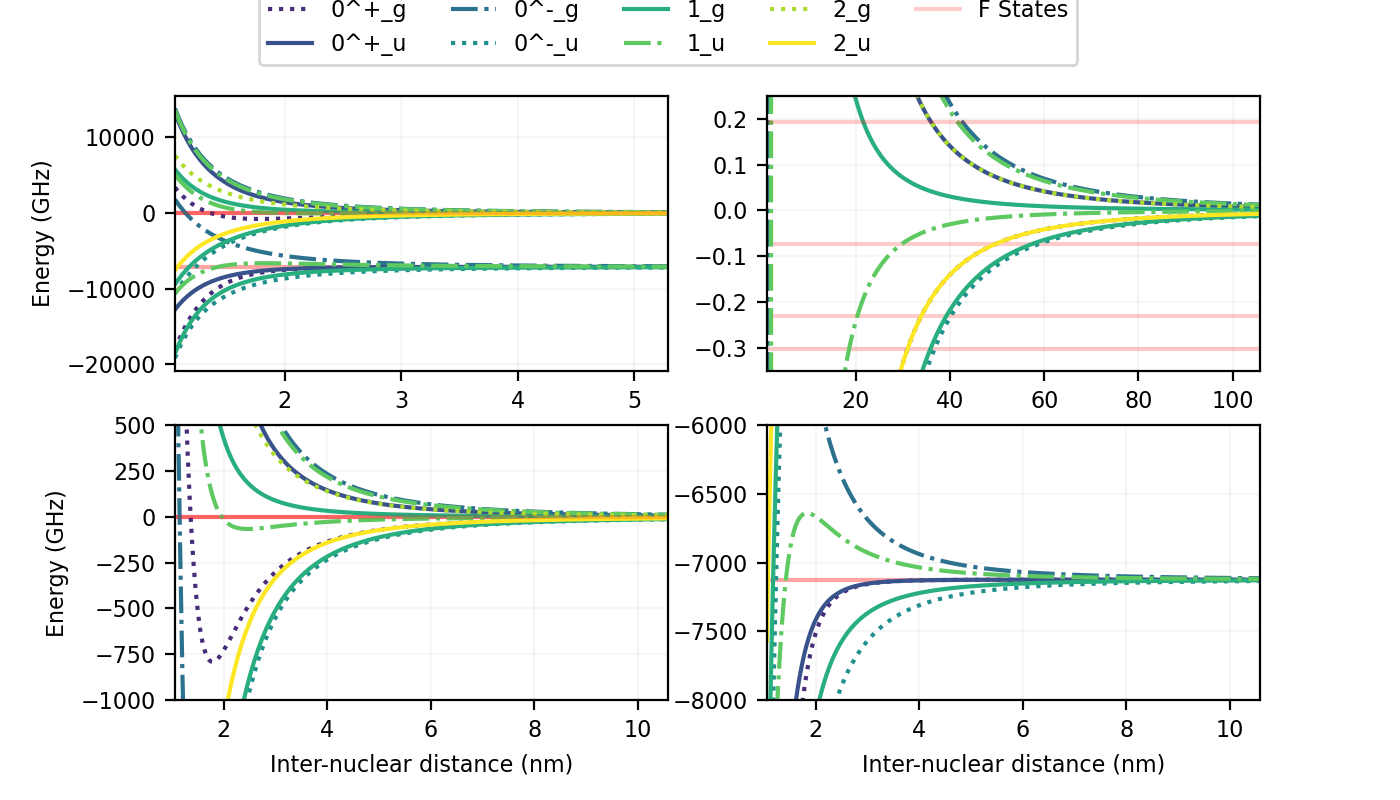
\includegraphics[width=\textwidth]{Movre-Pischler}
    \caption{The Movre-Pischler Potentials with various zooms.}
\end{figure}

% %%%%%%%%%%%%%%%%%%%%%%%%%%%%%%%%%%%%%%%%%%%%%%%%%%%%%%%%%%%%
% %%%%%%%%%%%%%%%%%%%%%%%%%%%%%%%%%%%%%%%%%%%%%%%%%%%%%%%%%%%%
\section{Rotation}
% %%%%%%%%%%%%%%%%%%%%%%%%%%%%%%%%%%%%%%%%%%%%%%%%%%%%%%%%%%%%
% %%%%%%%%%%%%%%%%%%%%%%%%%%%%%%%%%%%%%%%%%%%%%%%%%%%%%%%%%%%%

In general adding rotation to the problem complicates matters greatly. The Hamiltonian here is

\begin{equation}
H_R = \frac{\hat{N}^2}{2\mu R^2}
\end{equation}

$H_R$ doesn't commute with either $H_{BO}$ or $H_{FS}$, so at this point we have three hamiltonians in our main total Hamiltonian. Depending on $R$ and the rotational state, any of these hamiltonians can dominate, and so depending on their relative states different state bases should be used to describe the states. The different cases of which terms are strongest are called Hund's cases in the literature, and there are five of them labeled (a)-(e). $H_{BO}$ is diagonal in case (a) and case (b) states, $H_{FS}$ is diagonal in the case (c) states, and $H_R$ is diagonal in cases (d) and case (e). Therefore, since we have been working in the BO basis for all this work, the challenge of adding this to the hamiltonian to the calculation amounts to finding the transformation matrices which transform states from case (e), where $H_R$ is diagonal and easy to evaluate, to case (a). States in case (e) are described by quantum numbers $J, j, \ell, j_a, $ and $j_b$, therefore the matrix elements we need to calculate are $\langle J, j, \ell, j_a, j_b|J, L\Lambda\sigma S \Sigma\rangle$.

Depending on how strong the rotational couplings are compared to the Born-Oppenheimer interactions and the , some old quantum numbers are no longer good quantum numbers. The BO potentials are derived in case (a/b) (it's agnostic as to which), while the fine-structure potentials use the case (c) basis. In the case that rotation is very strong, one goes to case (d) or case (e). In basis E the good quantum numbers are $|J M_J c \Lambda S \Sigma \mathcal{P} \rangle $ where $\mathcal{P}$ describes the total parity of the state, and where $M_J$ is the projection of J on the relevtant rotational axis, \emph{not} the internuclear axis. We need to rotate this basis into the basis using projections along the internuclear axis. In general we do this with the \emph{Wigner D-Matrices} represented by the matrix elements $D^J_{M_J,\Omega}=\langle J,M_J|\mathcal{R}\{\alpha,\beta\gamma\}|J, \Omega\rangle$ where $\mathcal{R}\{\alpha,\beta\gamma\}$ are standard 3D rotation matrices with euler angles $\alpha, \beta,$ and $\gamma$. The original reference for this derivation is \cite{singer_theory_1983}, although Paul's notes explain the matter more clearly TBH. 
As usual, only the absolute value of the projection is expected to matter, so we will have to include the appropriatly superposition of the two $\Omega$ states. 
Therefore, we expect to be able to write the original basis in the form $|J M_J; L \Lambda L_a L_b; S \Sigma  S_1 S_2; \mathcal{P} \rangle=N(D^{J*}_{M_J\Omega}|L \Lambda L_1 L_2; S \Sigma S_1 S_2\rangle+pD^{J*}_{M_J-\Omega}|L -\Lambda L_1 L_2; S -\Sigma S_1 S_2\rangle)$. One can think about the symmetrization and normalization carefully and come to the conclusion that this must be
\begin{equation}
\begin{split}
|J M_J; L \Lambda L_a L_b; S \Sigma  S_1 S_2; \mathcal{P} \rangle=\\
\frac{1}{\sqrt{2-\delta_{\Lambda 0}\delta_{\Sigma 0}}}\sqrt{\frac{2J+1}{8\pi^3}}\bigg[&D^{J*}_{M_J\Omega}\{\alpha \beta \gamma\}|L \Lambda L_a L_b; S \Sigma S_a S_b\rangle\\
&+\mathcal{P}(-1)^{l_a+l_b+J-S}D^{J*}_{M_J-\Omega}\{\alpha \beta \gamma\}|L, -\Lambda L_a L_b; S, -\Sigma S_a S_b\rangle\bigg]
\end{split}
\end{equation}

We need to represent the $|j\Omega j_a j_b\rangle$ state in terms of the single particle states:
\begin{equation}
|L \Lambda L_1 L_2; S \Sigma S_1 S_2\rangle = \sum_{j, j_a, j_b} |j\Omega j_a j_b\rangle\langle j\Omega j_a j_b | L_a L_b \Lambda_a \Lambda_b; S\Sigma S_a S_b\rangle
\end{equation}

So we need to calculate these matrix elements between the states which are just going to end up giving us a ton of clebsch gordon coefficients: 
\begin{align}
&\langle j\Omega j_a j_b | L_a L_b \Lambda_a \Lambda_b; S\Sigma S_a S_b\rangle \\
= &\Bigg(\sum_{\Omega_a \Omega_b} C_{j_a j_b \Omega_a \Omega_b}^{j \Omega} \langle j_a j_b \Omega_a \Omega_b |\Bigg)|L_a L_b \Lambda_a \Lambda_b\rangle \Bigg(\sum_{\Sigma_a\Sigma_b} C_{S_a S_b \Sigma_a \Sigma_b}^{S \Sigma}| S_a S_b \Sigma_a \Sigma_b\rangle\Bigg)\\
=&\Bigg(\sum_{\Omega_a \Omega_b}C_{j_a j_b \Omega_a \Omega_b}^{j \Omega}\Big(\sum_{\Lambda_a\Sigma_a} C_{L_a S_a \Lambda_a \Sigma_a}^{j_a \Omega_a}\langle L_a S_a \Lambda_a \Sigma_a |\Big)\Big(\sum_{\Sigma_b\Lambda_b} C_{L_b S_b \Lambda_b \Sigma_b}^{j_b \Omega_b}\langle L_b S_b \Lambda_b \Sigma_b |\Big)\Bigg)\\
&\times|L_a L_b \Lambda_a \Lambda_b\rangle\Bigg(\sum_{\Sigma_a\Sigma_b} C_{S_a S_b \Sigma_a \Sigma_b}^{S \Sigma} | S_a S_b \Sigma_a \Sigma_b\rangle\Bigg)\\
=&\sum_{\Sigma_a \Sigma_b \Omega_a \Omega_b} 
C_{j_a j_b \Omega_a \Omega_b}^{j \Omega} 
C_{L_a S_a \Lambda_a \Sigma_a}^{j_a \Omega_a}
C_{L_b S_b \Lambda_b \Sigma_b}^{j_b \Omega_b} 
C_{S_a S_b \Sigma_a \Sigma_b}^{S \Sigma}\\
=&\sum_{L} \sqrt{\breve{S}\breve{j_a}\breve{j_b}\breve{L}} 
C_{L_a L_b \Lambda_a \Lambda_b}^{L \Lambda}
C_{L S \Lambda \Sigma}^{j \Omega}
\begin{Bmatrix}
L_a & S_a & j_a\\
L_b & S_b & j_b\\
L & S & j
\end{Bmatrix}\\
=&\sqrt{\breve{S}\breve{j_a}\breve{j_b}\breve{L}} 
C_{L S \Lambda \Sigma}^{j \Omega}
\begin{Bmatrix}
L_a & S_a & j_a\\
L_b & S_b & j_b\\
L & S & j
\end{Bmatrix}
\end{align}

(should redo to match the 9j definition) Here we have $\breve{x}=2x+1$ where $x$ is any angular momentum quantum number. We can see here that we have to be careful with the signs of the projections, as these will carry through to the clebsch gordon coefficient.  The term in curly brackets is known as the Wigner 9-j symbol - it evaluates to a constant. Where in the last step I used the fact that we know for atoms of interest for us there is only one value of L, specifically $L=L_b=1$ and $L_a=0$ to remove the superfluous clebsch gordon coefficient and sum over $L$. We need to rotate the single particle states. They can be rotated through the following relation:
\begin{equation}
|j\Omega j_a j_b\rangle = \sum_m |j m j_a j_b\rangle D^j_{m \Omega}\{\alpha\beta\gamma\}
\end{equation}

Therefore, equation 15 becomes...
\begin{equation}
\begin{split}
|J M_J; L \Lambda L_a L_b; S \Sigma  S_1 S_2; \mathcal{P} \rangle
\\
=&\frac{1}{\sqrt{2-\delta_{\Lambda 0}\delta_{\Sigma 0}}}\sqrt{\frac{2J+1}{8\pi^3}}\bigg[D^{J*}_{M_J\Omega}\{\alpha \beta \gamma\}|L \Lambda L_a L_b; S \Sigma S_a S_b\rangle
\\
+\mathcal{P}(-1)^{l_a+l_b+J-S}D^{J*}_{M_J-\Omega}\{\alpha \beta \gamma\}|L, -\Lambda L_a L_b; S, -\Sigma S_a S_b\rangle\bigg]
\frac{1}{\sqrt{2-\delta_{\Lambda 0}\delta_{\Sigma 0}}}
\sqrt{\frac{2J+1}{8\pi^3}}
\sum_{j, m_j, j_a, j_b} \bigg[D^{J*}_{M_J\Omega}\{\alpha \beta \gamma\}|j m j_a j_b\rangle D^j_{m \Omega}\{\alpha\beta\gamma\}
\\
+\mathcal{P}(-1)^{l_a+l_b+J-S}D^{J*}_{M_J-\Omega}\{\alpha \beta \gamma\}|j m j_a j_b\rangle D^j_{m,-\Omega}\{\alpha\beta\gamma\}\bigg]
\\
\sqrt{\breve{S}\breve{j_a}\breve{j_b}\breve{L}} C_{L S \Lambda \Sigma}^{j \Omega}
\begin{Bmatrix}
L_a & S_a & j_a\\
L_b & S_b & j_b\\
L & S & j
\end{Bmatrix}
\end{split}
\end{equation}

There are a couple important relations for the Wigner D matrix here: 

\begin{equation}
\begin{split}
\sqrt{\frac{4\pi}{2\ell+1}}Y_{\ell \mu}\{\beta, \alpha\}=\sqrt{\frac{4\pi}{2\ell+1}}|\ell\mu\rangle=D^{\ell *}_{\mu 0} \{\alpha \beta \gamma\}\\
D^{J*}_{M_J \Omega}\{\alpha,\beta,\gamma\} =(-1)^{M_J-\Omega} D_{-M_J,-\Omega}\{\alpha,\beta,\gamma\}\\
D_{-M_j,-\Omega}^{J}\{\alpha,\beta,\gamma\}
D_{m_j \Omega}^{j}\{\alpha,\beta,\gamma\} 
= \sum_{\ell=|j-j'|}^{j+j'}
C_{J,-M_J j m_j}^{\ell, -M_J + m_j}
C_{J,-\Omega j \Omega}^{\ell 0}
D^{\ell}_{-M_J + m_j,0}\{\alpha,\beta,\gamma\}
\end{split}
\end{equation}

We can use these on equation 25. Note that since $\hat{J}=\hat{j}+\hat{N}$, we have $M_J-m_j=\mu$. :
\begin{equation}
\begin{split}
|J M_J; L \Lambda L_a L_b; S \Sigma  S_1 S_2; \mathcal{P} \rangle=\\
\frac{1}{\sqrt{2-\delta_{\Lambda 0}\delta_{\Sigma 0}}}
\frac{1}{2\pi}
\sum_{j, m_j, j_a, j_b} \sum_{\ell=|j-j'|}^{j+j'} \bigg[
&C_{J,-M_J j m_j}^{\ell, -\mu}
C_{J,-\Omega, j \Omega}^{\ell 0}
(-1)^{M_j-\Omega}|\ell\mu j m j_a j_b\rangle\\
&+\mathcal{P}(-1)^{l_a+l_b+J-S}
C_{J,-M_J j m_j}^{\ell, -\mu}
C_{J\Omega j,-\Omega}^{\ell 0}
(-1)^{M_j+\Omega}|\ell\mu j m j_a j_b\rangle\bigg]\\
\times\sqrt{\breve{S}\breve{j_a}\breve{j_b}\breve{L}} 
C_{L \Lambda S \Sigma}^{j \Omega}
\begin{Bmatrix}
L_a & S_a & j_a\\
L_b & S_b & j_b\\
L & S & j
\end{Bmatrix}
\end{split}
\end{equation}

Note that there are some very funny clebsch gordon coefficients here that aren't quite what I want. I want to go from $|\ell\mu jm_j\rangle\rightarrow|J M_J \ell j\rangle$, so I need clebsch gordon coefficients of the form $C_{\ell \mu j m_j}^{J M_J}$, not the ones I have here. These are related though:

\begin{equation}
\begin{split}
C_{\ell \mu j m_j}^{J M_J} = \langle\ell \mu j m_j |J M_J \rangle = (-1)^{j+m_j}\sqrt{\frac{\breve{J}}{\breve{\ell}}}\langle J, -M_J j m_j |\ell, -\mu \rangle\\
C_{J\Omega j,-\Omega}^{\ell 0} = (-1)^{J+j-\ell}C_{J,-\Omega j\Omega}^{\ell 0}\\
C_{J\Omega j,-\Omega}^{\ell 0} = (-1)^{J+j-\ell}C_{j,-\Omega J\Omega}^{\ell 0}\\
\end{split}
\end{equation}

This looks promising because it corrects the signs, but it looks less promising because of the extra funny factor there. But let's try it for a moment:

\begin{equation}
\begin{split}
&|J M_J; L \Lambda L_a L_b; S \Sigma  S_1 S_2; \mathcal{P} \rangle
\\
&=\frac{1}{\sqrt{2-\delta_{\Lambda 0}\delta_{\Sigma 0}}}
\frac{1}{2\pi}(-1)^{j+m_j+M_J-\Omega}
\sum_{j, m_j, j_a, j_b} \sum_{\ell=|j-j'|}^{j+j'} C_{\ell \mu j m_j}^{J M_J}\bigg[
C_{J,-\Omega, j \Omega}^{\ell 0}
|\ell\mu j m j_a j_b\rangle
\\
&+\mathcal{P}(-1)^{l_a+l_b+J-S}
C_{J\Omega j,-\Omega}^{\ell 0}
|\ell\mu j m j_a j_b\rangle\bigg]
\\
&\times\sqrt{\breve{S}\breve{j_a}\breve{j_b}\breve{L}} 
C_{L \Lambda S \Sigma}^{j \Omega}
\begin{Bmatrix}
L_a & S_a & j_a\\
L_b & S_b & j_b\\
L & S & j
\end{Bmatrix}
\\
&=\frac{1}{\sqrt{2-\delta_{\Lambda 0}\delta_{\Sigma 0}}}
\frac{1}{2\pi}(-1)^{j+m_j+M_J-\Omega}
\sum_{j, m_j, j_a, j_b} \sum_{\ell=|j-j'|}^{j+j'} C_{\ell \mu j m_j}^{J M_J}C_{j,-\Omega J\Omega}^{\ell 0}(-1)^{2J+2j-2\ell}\bigg[
|\ell\mu j m j_a j_b\rangle
\\
&+\mathcal{P}(-1)^{l_a+l_b+J-S}(-1)^{\ell-J-j}
C_{J\Omega j,-\Omega}^{\ell 0}
|\ell\mu j m j_a j_b\rangle\bigg]
\\
&\times\sqrt{\breve{S}\breve{j_a}\breve{j_b}\breve{L}} 
C_{L \Lambda S \Sigma}^{j \Omega}
\begin{Bmatrix}
L_a & S_a & j_a\\
L_b & S_b & j_b\\
L & S & j
\end{Bmatrix}\\
&=\frac{1}{\sqrt{2-\delta_{\Lambda 0}\delta_{\Sigma 0}}}
\frac{1}{2\pi}(-1)^{j+m_j+M_J-\Omega}
\sum_{j, m_j, j_a, j_b} \sum_{\ell=|j-j'|}^{j+j'} C_{\ell \mu j m_j}^{J M_J}C_{j,-\Omega J\Omega}^{\ell 0}(-1)^{2J+2j-2\ell}
\\
&\bigg[1+\mathcal{P}(-1)^{l_a+l_b+\ell-S-j}\bigg]
|\ell\mu j m j_a j_b\rangle
\times\sqrt{\breve{S}\breve{j_a}\breve{j_b}\breve{L}} 
C_{L \Lambda S \Sigma}^{j \Omega}
\begin{Bmatrix}
L_a & S_a & j_a\\
L_b & S_b & j_b\\
L & S & j
\end{Bmatrix}\\
\end{split}
\end{equation}


And finally summing over the clebch gordon coefficient using normal addition of angular momentum definitions:
\begin{equation}
\begin{split}
|J M_J; L \Lambda L_a L_b; S \Sigma  S_1 S_2; \mathcal{P} \rangle=\\
\frac{1}{\sqrt{2-\delta_{\Lambda 0}\delta_{\Sigma 0}}}
\frac{1}{2\pi}
\sum_{j, m_j, j_a, j_b} \bigg[
&(-1)^{M_j-\Omega}|J M_J \ell j j_a j_b\rangle\\
&+(1-\delta_{\Lambda 0} \delta_{\Sigma 0} ) (-1)^{\mathcal{P}+J-S+\sigma}
(-1)^{M_j+\Omega}|J M_J \ell j j_a j_b\rangle\bigg]\\
\times\sqrt{\breve{S}\breve{j_a}\breve{j_b}\breve{L}} 
C_{Jj, -\Omega \Omega}^{\ell 0}
C_{L S \Lambda \Sigma}^{j \Omega}
\begin{Bmatrix}
L_a & S_a & j_a\\
L_b & S_b & j_b\\
L & S & j
\end{Bmatrix}
\end{split}
\end{equation}


And then there seems to be some crucial step missing to get to the final result. I'm not sure how to make sense of the weird clebsch Gordon sums and the fact that we seem to be getting some sort of $J+j$ terms from the wigner D matrix identities, which seem unphysical since the rotation operator is $J-j$. I'm suspicious that the weird rotations on the original states should give the $Jmj\ell j_a j_b$ states in equation II.12 in my main reference here, but I don't know how that comes about. 

In the end, the conversion between case (a) and case (e) is then given by the following:
\begin{equation}
\langle j \ell j_a j_b | \Lambda S \Sigma p\rangle_J = (-1)^{\ell-\Omega-J} \frac{1+(-1)^{L_b+\ell+p}(1-\delta_{\Lambda,0}\delta_{\Sigma,0})}{\sqrt{2-\delta_{\Lambda,0}\delta_{\Sigma,0}}}\sqrt{\breve{S}\breve{j_a}\breve{j_b}\breve{L}} C_{j,-\Omega J\Omega}^{\ell 0}C_{L\Lambda S\Sigma}^{j\Omega}
\begin{Bmatrix}
L_a & S_a & j_a\\
L_b & S_b & j_b\\
L & S & j
\end{Bmatrix}
\end{equation}

This nasty relation allows you to calculation transformation matrices to convert all the case (e) basis states to case (a) in order to evaluate the hamiltonian for each value of $\ell$ and as a function of R. For the record I'm not sure using the 9j symbol here really makes things simpler, but okay. 

For a given value of J, states can have either positive or negative total parity. It turns out that the results of these calculations result in pairs of closely spaced rotational energy levels which have different pairity, and so each state gets an additional label. States with parities $(-1)^J$ are said to have "e" parity, and states with pairities $-(-1)^J$ are said to have "f" parity. This scheme ensures that each state in the doublet has different such parity, and as well the "e" and "f" are independent of the hunds case basis used. In other words, the matrix elements above do not mix states of different "e/f" parity. This parity label has historically fluctuated and been the source of confusion in the field \cite{hornkohl_parity_2017,brown_labeling_1975}.

In the end, I can use this calculation to calculate the rotational couplings, as shown in figure (2)
\begin{figure}
  \centering
    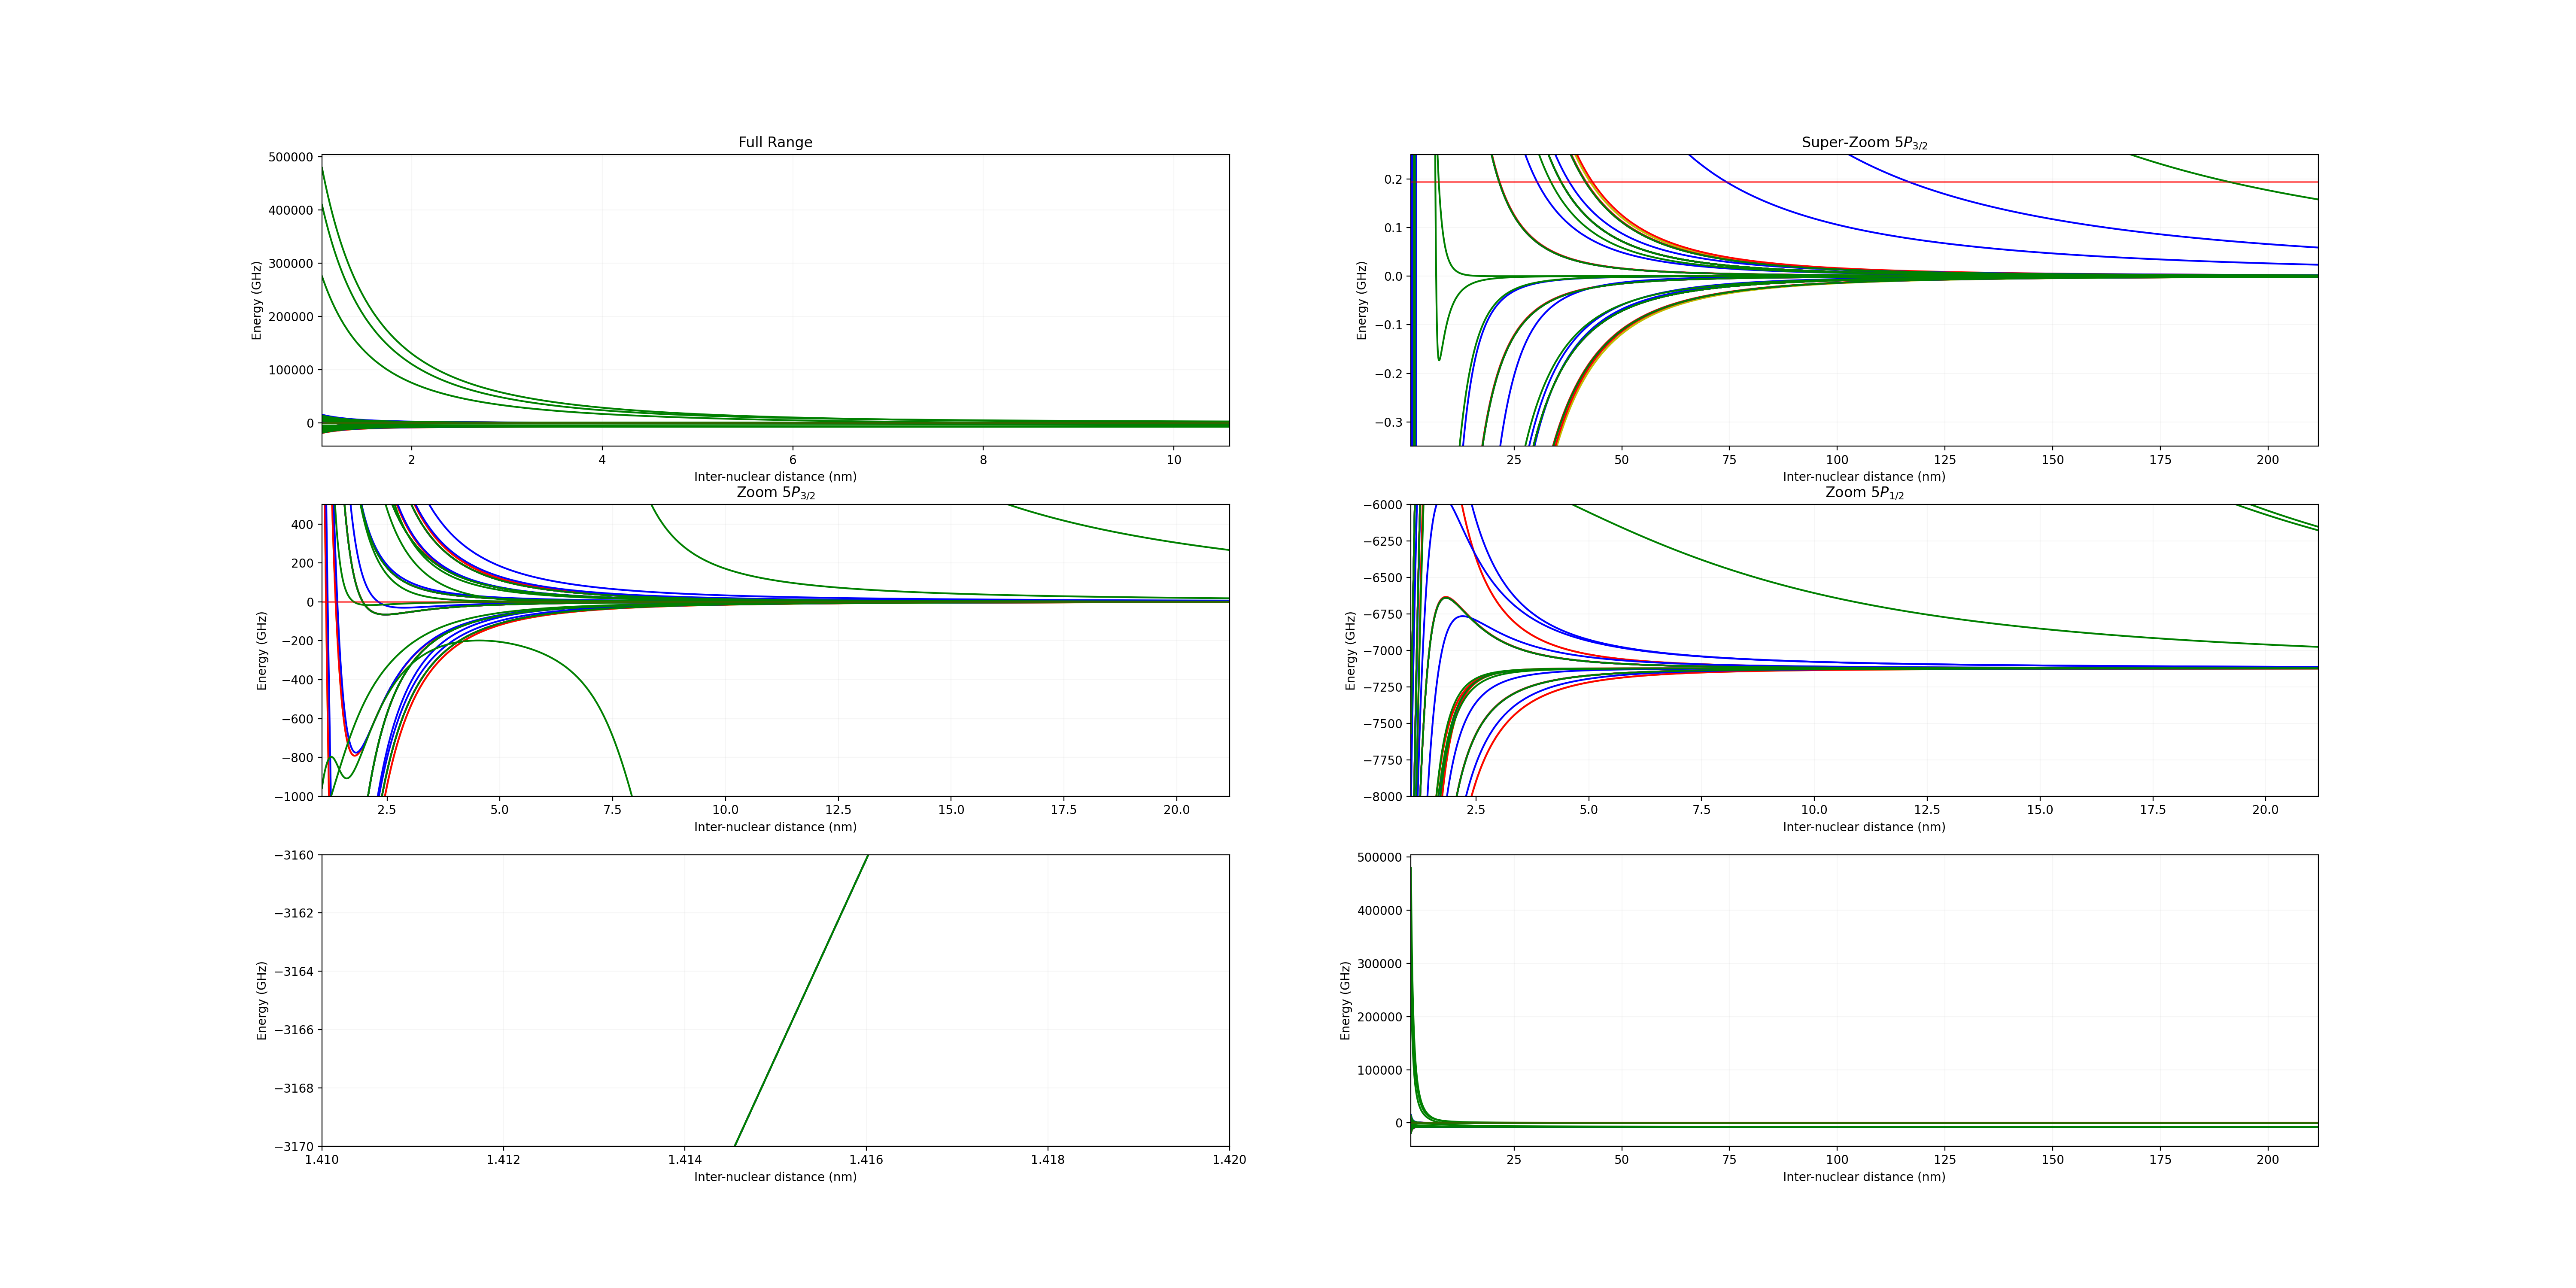
\includegraphics[width=\textwidth]{Movre-Pischler-Super-Rotating}
    \caption{The Movre-Pischler Potentials with ridiculously large rotational couplings. Values are $\ell=3$ (yellow) $\ell=10$ (Blue), $\ell=100$ (red), and $\ell=1000$ (green). }
\end{figure}

% %%%%%%%%%%%%%%%%%%%%%%%%%%%%%%%%%%%%%%%%%%%%%%%%%%%%%%%%%%%%
% %%%%%%%%%%%%%%%%%%%%%%%%%%%%%%%%%%%%%%%%%%%%%%%%%%%%%%%%%%%%
\section{Hyperfine Structure} 
% %%%%%%%%%%%%%%%%%%%%%%%%%%%%%%%%%%%%%%%%%%%%%%%%%%%%%%%%%%%%
% %%%%%%%%%%%%%%%%%%%%%%%%%%%%%%%%%%%%%%%%%%%%%%%%%%%%%%%%%%%%

\begin{figure}
  \centering
    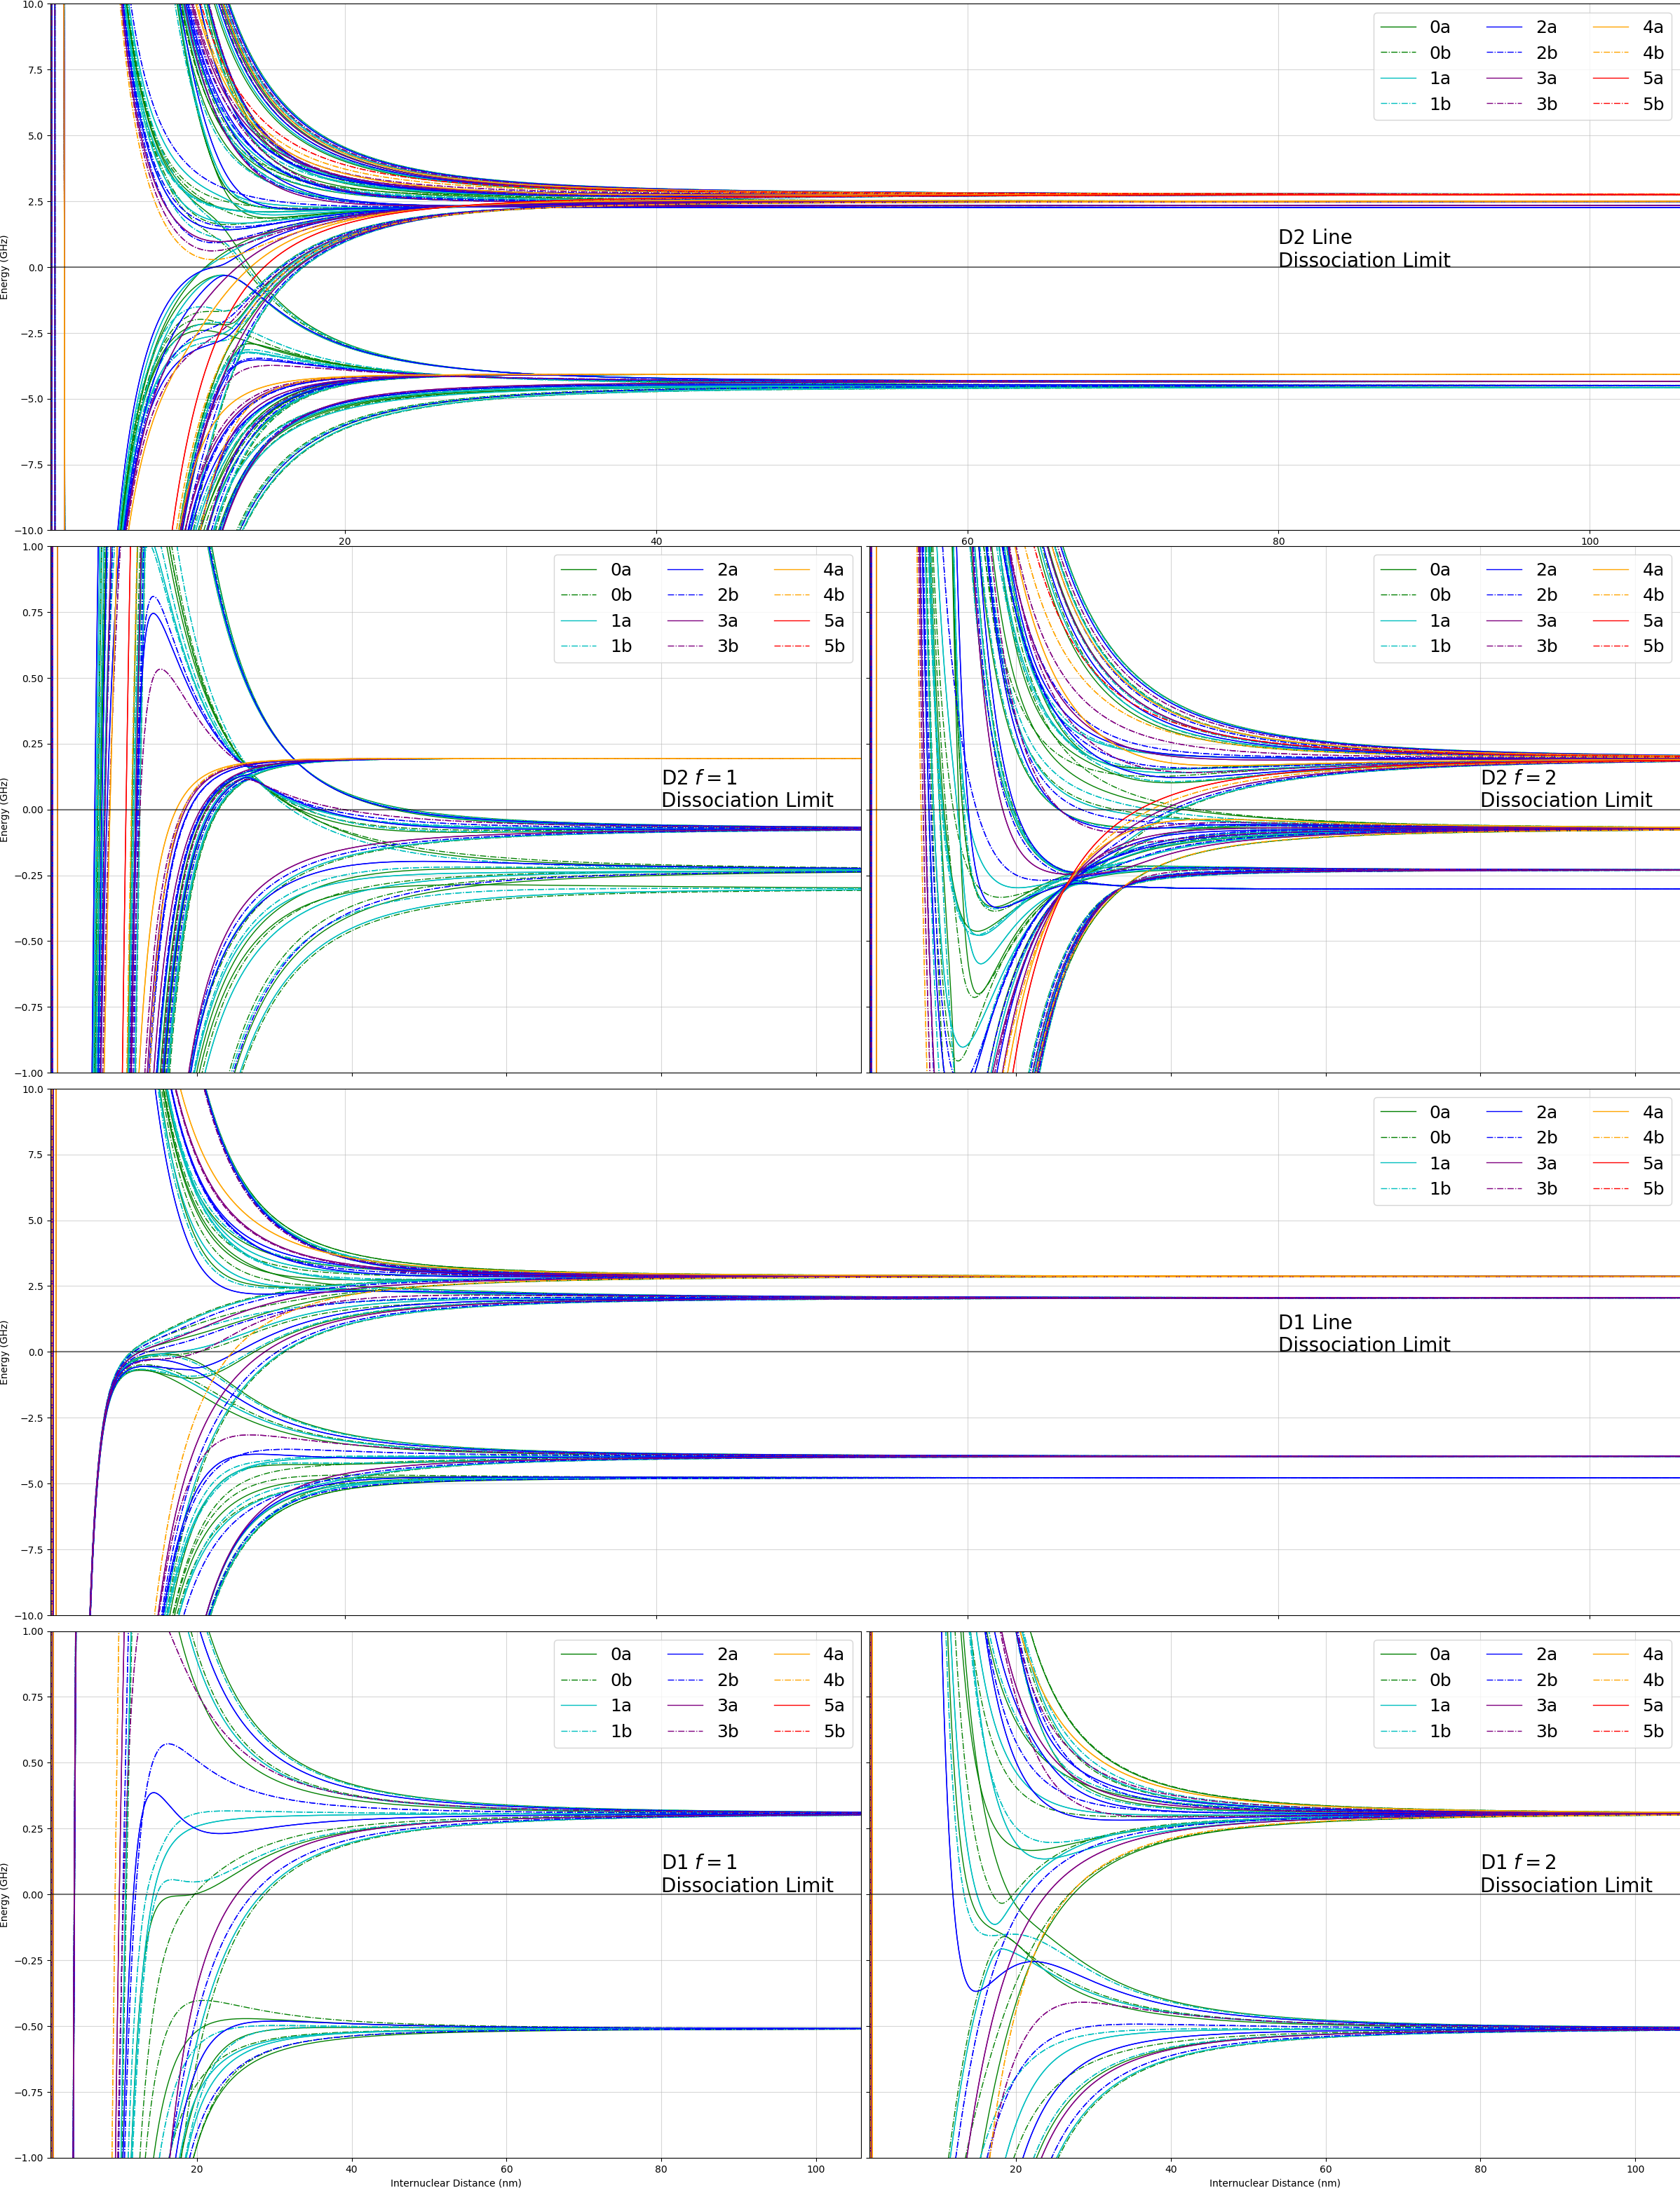
\includegraphics[width=\textwidth]{Hyperfine_Splitting_Big_Picture}
    \caption{Hyperfine Splittings, big picture. }
\end{figure}



Adding hypefine coupling, $H_{hf} = A(\hat{I}_a\cdot\hat{J}_a+\hat{I}_b\cdot\hat{J}_b)$ breaks the g/u symmetry because the molecule is generally not symmetric about the internuclear plane when the two nuclei can have different spins. This leaves only the total parity, $\phi$, and the symmetry about a plane that contains the internuclear axis for $\phi=0$ states. The Rubidium dissociation paper\cite{kemmann_near-threshold_2004} discusses these symmetries some. Otherwise the calculations are fairly straightforward, mostly just involving an expansion of the basis used to calculate the eigenenergies of the total hamiltonian. Figures 3,4, and 5 show the results of these calculations using Rb87 numbers. Note that all the states with $\phi\neq 0$ are doubly degenerate corresponding to the positive and negative phi states. The legends of the figures here report the value of $\phi$ and the number of non-degenerate states in parentheses. 
\begin{figure}
  \centering
    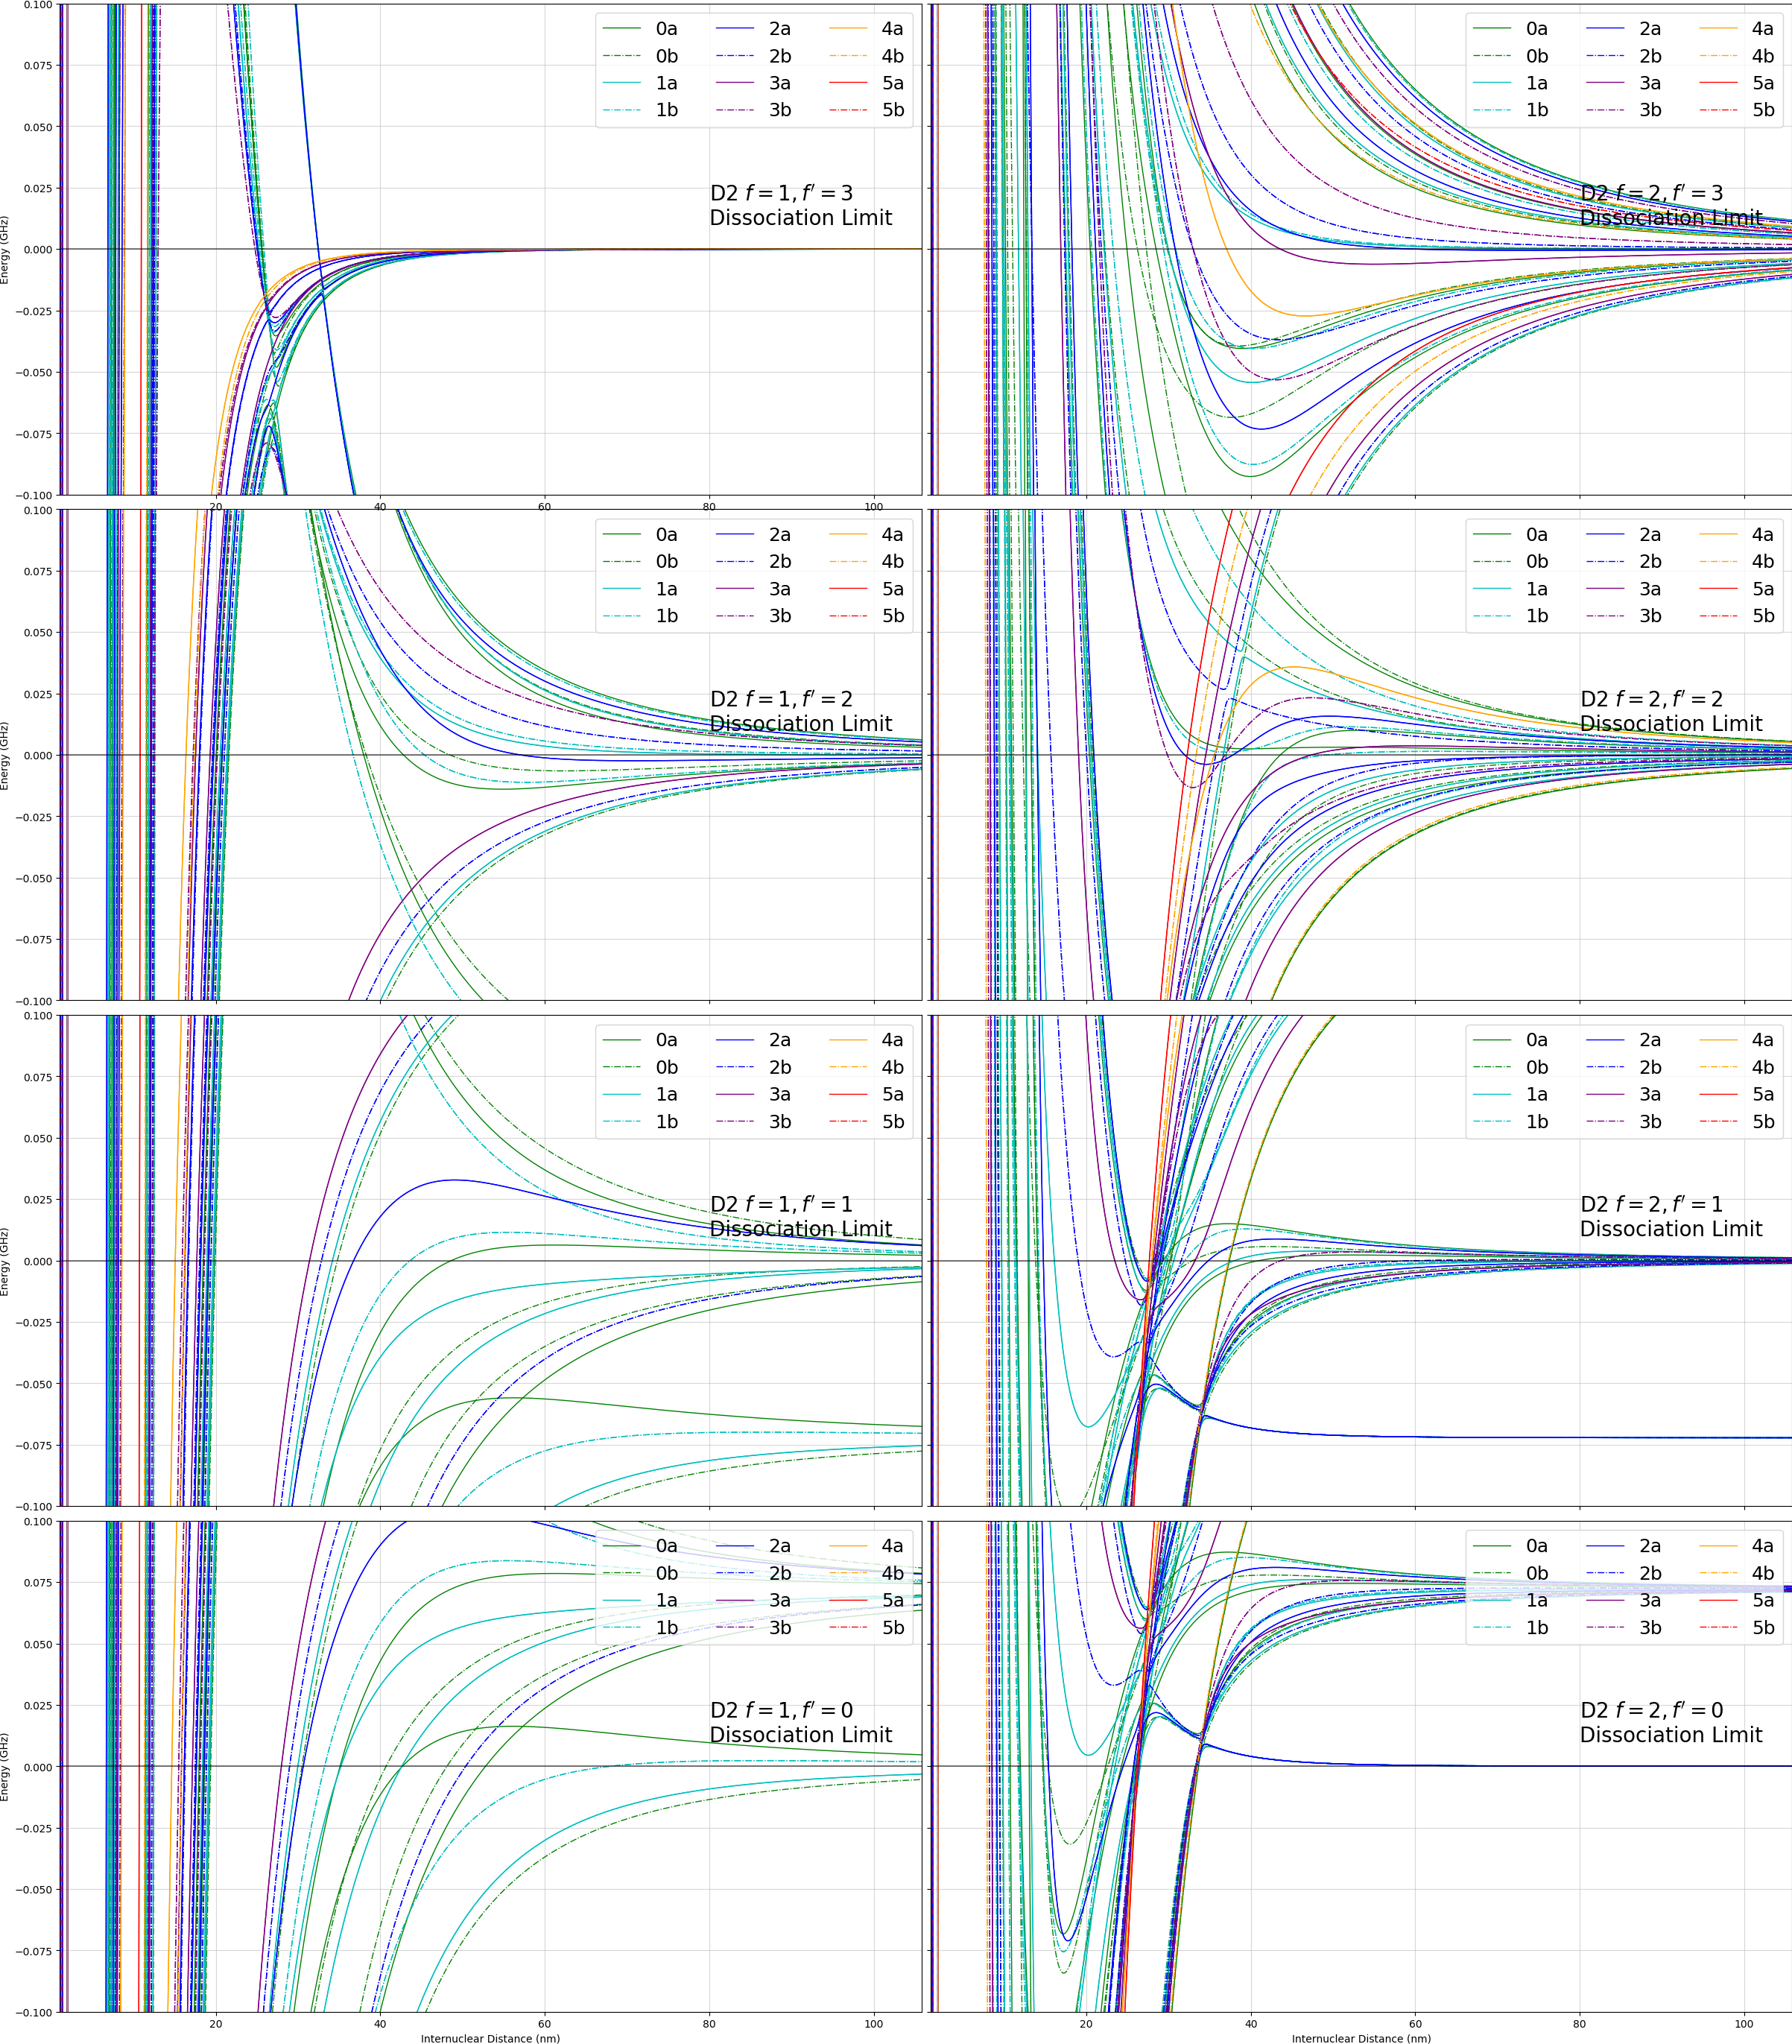
\includegraphics[width=\textwidth]{Hyperfine_Splitting_D2_Zoom}
    \caption{Hyperfine Splittings, D2 Line Manifolds. }
\end{figure}

I have yet to track down how to identify states of these other symmetries. This is I think a key crucial next step.

\begin{figure}
  \centering
    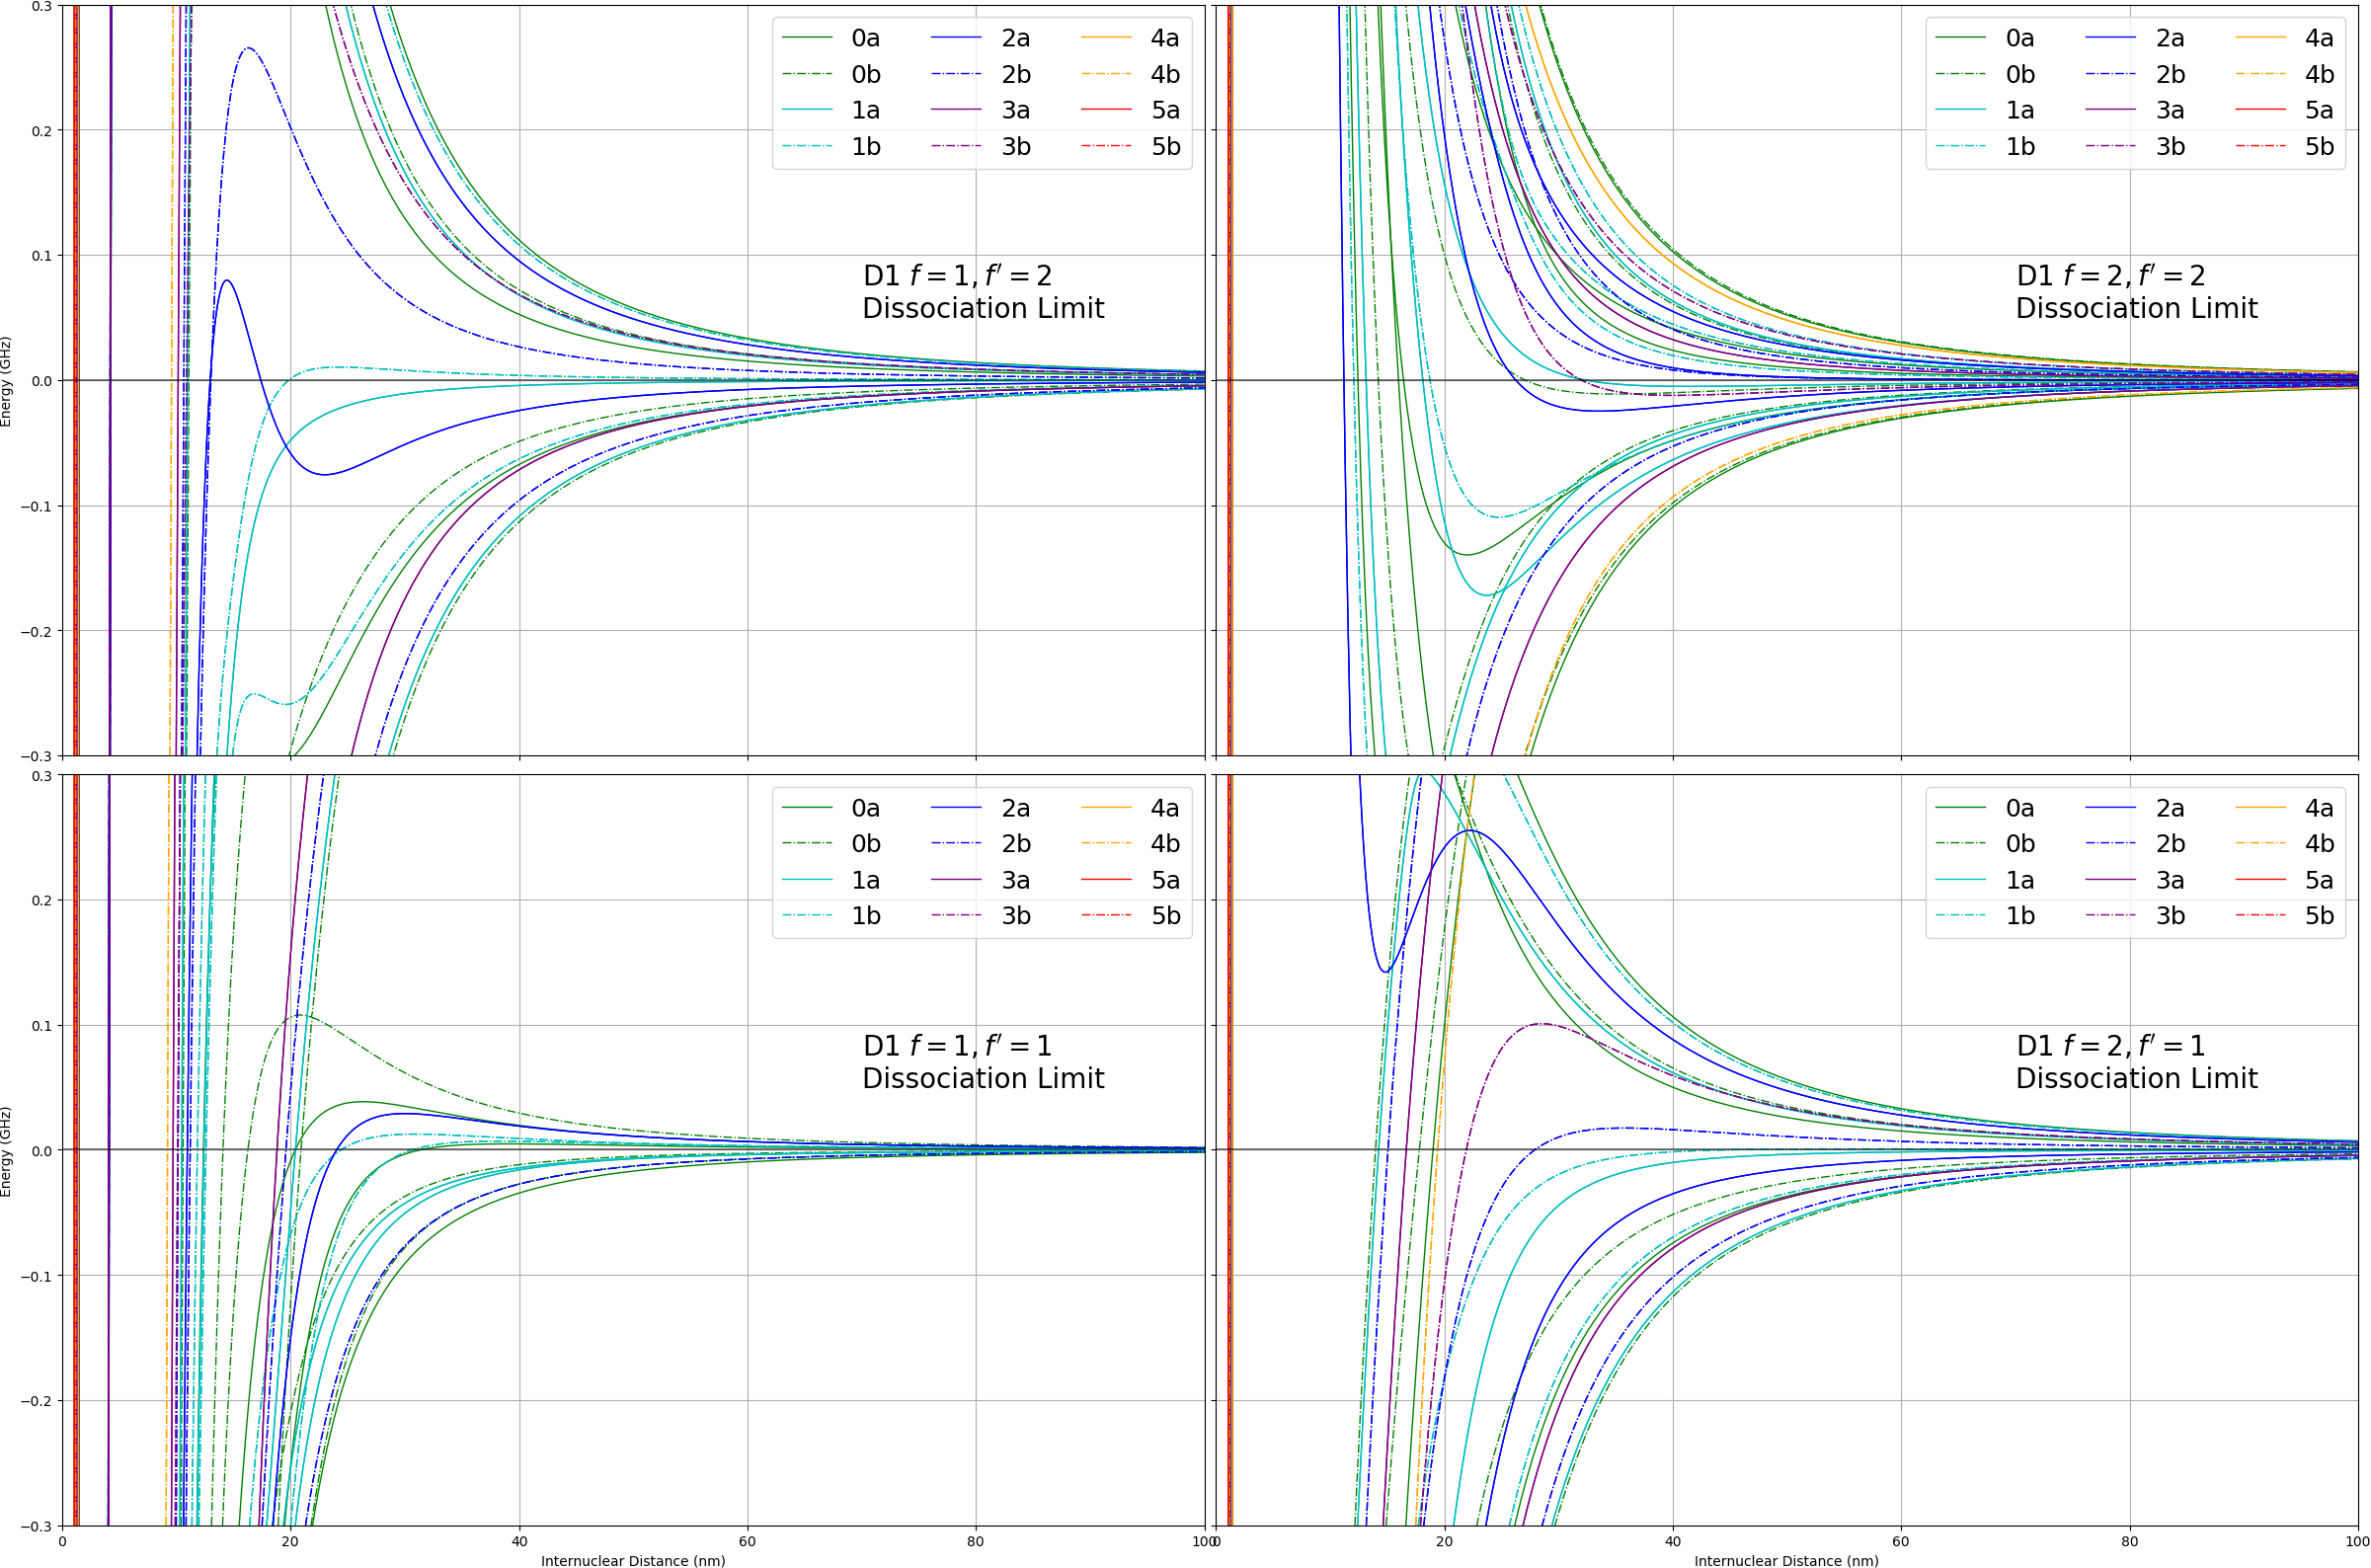
\includegraphics[width=\textwidth]{Hyperfine_Splitting_D1_Zoom}
    \caption{Hyperfine Splittings, D1 Line Manifolds. }
\end{figure}

Evaluating the coupling constant is slightly more tricky than the fine-structure constant $A(\hat{I}\cdot\hat{J})$ because there are more manifolds for the hyperfine constant. The coupling constant evidently takes different values for the different manifolds. For example, in Rubidium, the ground state splitting is 6.8 GHz, while the splitting of the D1 line is about 800MHz. As such, to evaluate the hyperfine coupling, I simply forced the diagonal elements of the hyperfine coupling matrix in the F basis to match the experimental values. (The operator is diagonal in this basis so there are no off-diagonal values to consider).  This includes explicitly plugging in the values for the 4 different hyperfine manifolds on the D2 transition - without doing this and if trying to parameterize the splitting by a single value, the dissociation energies were off by ~ 10MHz from their experimental values. 

% %%%%%%%%%%%%%%%%%%%%%%%%%%%%%%%%%%%%%%%%%%%%%%%%%%%%%%%%%%%%
% %%%%%%%%%%%%%%%%%%%%%%%%%%%%%%%%%%%%%%%%%%%%%%%%%%%%%%%%%%%%
\section{Hyperfine Structure With Rotation} 
% %%%%%%%%%%%%%%%%%%%%%%%%%%%%%%%%%%%%%%%%%%%%%%%%%%%%%%%%%%%%
% %%%%%%%%%%%%%%%%%%%%%%%%%%%%%%%%%%%%%%%%%%%%%%%%%%%%%%%%%%%%

This section will be mostly based off of Pauls notes, although Paul did not quite finish this section of the paper, so some results at the end will have to be derived and checked themselves. These notes are not complete, however, I should make that clear. Work in progress, I haven't gotten rotational potentials with hyperfine splittings complete yet. 

Paul's notes make it somewhat more clear where all the bases are coming from. 

\begin{equation}
\begin{split}
\text{Case (m):} |\ell \mu, c_a f_a m_{f_a}, c_b f_b m_{f_b}\rangle_m = |c_a f_a m_{f_a}, c_b f_b m_{f_b}\rangle\otimes Y_{\ell \mu}\\
\text{Case (e):} |F M_F, \ell f, c_a f_a, c_b f_b\rangle_e\\
\text{In Between (e) and (m):} |\ell\mu, f m_f, c_a f_a, c_b f_b\rangle_{??}
\end{split}
\end{equation}

Working with case (a) is slightly more tricky because we want to have states of good total parity. We start with

\begin{equation}
|F M_F, c \Lambda, S \Sigma, I \iota\rangle = \sqrt{\frac{2F+1}{8\pi^2}} D_{M_F,\phi}^{* F}\{\alpha \beta \gamma\} |c\Lambda S\Sigma I \iota\rangle
\end{equation}

where $D_{M_F,\phi}^{* F}\{\alpha \beta \gamma\}$ si the complex conjugate of the Wigner Rotation matrix for angles $\alpha, \beta, $ and $\gamma$, which are arbitrary angles in the present context. However, this is surprisingly not a state of good total parity, so instead we form a linear combination of these states with appropriate pairty, and we get our case a basis:

\begin{equation}
\begin{split}
|F M_F c \Lambda S \Sigma I \iota p\rangle_{(a)} = &\frac{1}{\sqrt{2-\delta_{\Lambda 0}\delta{\Sigma 0}\delta_{\iota 0}}} \sqrt{\frac{2F+1}{8\pi^2}}\\
&\times\Bigg[D_{M_F,\phi}^{* F}\{\alpha \beta \gamma\} |c\Lambda ;S\Sigma; I \iota\rangle
+p(-1)^{l_a+l_b+F-I-S}D_{M_F,\phi}^{* F}\{\alpha \beta \gamma\} |c-\Lambda; S,-\Sigma; I, -\iota;\rangle\Bigg]
\end{split}
\end{equation}

I'm somewhat confused about the F in the ket here, it almost seems like self-contradictory notation, I should think about this more. 

It's only at large R that the BO states gain good values for the quantum numbers $l_a, l_b$. As such, it's only as $R\rightarrow\infty$ that

\begin{equation}
\begin{split}
|c\Lambda S \Sigma I \iota\rangle = \sum_{\Lambda_a, \Lambda_b}|c_a L_a \Lambda_a \rangle |c_b L_b \Lambda_b\rangle |S\Sigma\rangle |I\iota\rangle\langle\Lambda_a \Lambda_b|c\Lambda\rangle\\
|c_a L_a\Lambda_a\rangle|c_b L_b \Lambda_b\rangle|S\Sigma\rangle|I\iota\rangle
=\sum_{f,f_a,f_b} |f\phi c_a f_a c_b f_b \rangle \langle f\phi f_a f_b | \Lambda_a \Lambda_b S\Sigma I \iota \rangle
\\
|f\phi c_a f_a c_b f_b\rangle
=\sum_{m_f} D_{m_f\phi}^{f}|f m_f c_a f_a c_b f_b\rangle
\end{split}
\end{equation}

There are 6 basic angular momentum and multiple ways to couple them to construct states of total angular momentum $f$. As there are so many angular momentum, it seems probably possible to write this big matrix element in terms of the 15j symbols, but there is vanishingly little resources on such symbols, so the better approach is to use the 9j symbols for the coupling of 4 angular momentum. 

In general, suppose you have 4 angular momentum $j_i, i\in\{1,2,3,4\}$. Then, denote $\hat{j}_{ij}=\hat{j}_i+\hat{j}_j$, and $j_{1234}\equiv j_*$ for brevity. There is a common matrix element to consider between the coupling of these four angular momentum:

\begin{equation}
\langle j_{*} m_{j_{*}} j_{12}j_{34}|j_{*} m_{j_{*}}j_{13}j_{24}\rangle
\equiv\sqrt{\breve{j}_{12}\breve{j}_{34}\breve{j}_{13}\breve{j}_{24}}
\begin{Bmatrix}
j_1 & j_2 & j_{13}\\
j_3 & j_4 & j_{34}\\
j_{13} & j_{24} & j_{*}\\
\end{Bmatrix}
\end{equation} 

In the case here, there are two ways to construct the total electronic angular momentum $j$ (not using general notation here). We have $\hat{j}=\hat{l}_a+\hat{s}_a+\hat{l}_b+\hat{s}_b$, and we can first couple the two orbitatal angular momentums and spins to create states $|jm_j L S l_1 l_2 s_1 s_2 \rangle\equiv|j m_j L S\rangle$, or we can construct the individual electronic angular momentum first and create states $|j m_j j_1 j_2 l_1 s_1 l_2 s_2\rangle\equiv|j m_j j_1 j_2\rangle$. Similarly, we have four angular momentum $j_a, j_b, i_a, $ and $i_b$ to construct states of good $f$ in two critical ways to create two bases: $|f m_f j I\rangle$ or $|f m_f f_a f_b\rangle$. This is going to lead to two wigner 9j symbols. And this is suggestive that we are looking to construct the matrix elements $\langle f m_f f_1 f_2 | f m_f j I\rangle$ and $\langle j m_j j_1 j_2| j m_J L S\rangle$ out of the given matrix element, both of which will reduce to clesch gordon coefficients. From here, it's just basic angular momentum algebra to get to the desired result. 

\begin{equation}
\begin{split}
\langle f \phi f_a f_b |\Lambda_a \Lambda_b S\Sigma I\iota\rangle
\xrightarrow{R\rightarrow\infty}
\langle f \phi f_a f_b |l_a\Lambda_a l_b\Lambda_b S\Sigma I\iota\rangle\\
= \langle f \phi f_a f_b | \Bigg(\sum_{L} C^{L\Lambda}_{l_a \Lambda_a, l_b \Lambda_b} |L \Lambda\rangle\Bigg) | S\Sigma I\iota\rangle\\
= \sum_{L} C^{L\Lambda}_{l_a \Lambda_a, l_b \Lambda_b} \langle f \phi f_a f_b | \Big(\sum_{j}C_{L\Lambda S\Sigma}^{j\Omega} |j\Omega L S\rangle\Big) | I\iota\rangle\\
= \sum_{L, j} C^{L\Lambda}_{l_a \Lambda_a, l_b \Lambda_b} C_{L\Lambda S\Sigma}^{j\Omega} \langle f \phi f_a f_b | \Bigg(\sum_{j_1 j_2} |j\Omega j_1 j_2 \rangle\langle j\Omega j_1 j_2 |j\Omega L S\rangle\Bigg) | I\iota\rangle\\
= \sum_{L, j, j_1 j_2} 
C^{L\Lambda}_{l_a \Lambda_a, l_b \Lambda_b} 
C_{L\Lambda S\Sigma}^{j\Omega} 
\langle f \phi f_a f_b | |j\Omega j_1 j_2 \rangle | I\iota\rangle
\sqrt{\breve{j}_1\breve{j_2}\breve{L}\breve{S}}
\begin{Bmatrix}
l_a & s_a & j_a\\
l_b & s_b & j_b\\
L & S & j
\end{Bmatrix}\\
= \sum_{L, j, j_1 j_2} 
C^{L\Lambda}_{l_a \Lambda_a, l_b \Lambda_b} 
C_{L\Lambda S\Sigma}^{j\Omega} 
\langle f \phi f_a f_b | \Bigg(\sum_{f'} C_{j\Omega I \iota}^{f' \phi} |f' \phi j I\rangle\Bigg)
\sqrt{\breve{j}_1\breve{j_2}\breve{L}\breve{S}}
\begin{Bmatrix}
l_a & s_a & j_a\\
l_b & s_b & j_b\\
L & S & j
\end{Bmatrix}\\
= \sum_{L, j, j_1 j_2} 
C^{L\Lambda}_{l_a \Lambda_a, l_b \Lambda_b} 
C_{L\Lambda S\Sigma}^{j\Omega} 
 C_{j\Omega I \iota}^{f \phi}
\langle f \phi f_a f_b |f \phi j I\rangle
\sqrt{\breve{j}_1\breve{j_2}\breve{L}\breve{S}}
\begin{Bmatrix}
l_a & s_a & j_a\\
l_b & s_b & j_b\\
L & S & j
\end{Bmatrix}\\
= \sum_{L, j, j_1 j_2} 
\bigg(
C^{L\Lambda}_{l_a \Lambda_a, l_b \Lambda_b} 
C_{L\Lambda S\Sigma}^{j\Omega} 
C_{j\Omega I \iota}^{f \phi}
\bigg)
\sqrt{\breve{j}_1\breve{j_2}\breve{f}_1\breve{f_2}
\breve{L}\breve{S}\breve{J}\breve{I}}
\begin{Bmatrix}
l_a & s_a & j_a\\
l_b & s_b & j_b\\
L & S & j
\end{Bmatrix}
\begin{Bmatrix}
j_a & i_a & f_a\\
j_b & i_b & f_b\\
j & I & f
\end{Bmatrix}
\end{split}
\end{equation}

Now we can really appreciate the breve :) This algebra is easy to talk through although maybe a bit much to walk through by yourself. But there are a couple critical steps. In the third line, I change basis from $|J\Omega L S\rangle$ to $|J\Omega j_1 j_2\rangle$ using the 9j symbol transformation discussed above. This probably isn't necessary, persay, but without this we might have to introduce unnatural looking $L+i_a$ and $S+i_b$ quantum numbers. when I combine j and I to form f kets in the 5th line, I use a a prime'd quantum number $f'$ just to emphasize that at this point in the calculation this can take different values than the $f$ in the bra. Then the $f'$ disappears because the $\langle f|f'\rangle$ terms are always going to be $\delta_{f,f'}$, killing all terms in the sum except one. The last line of this equation is equation (21) is paul's notes. The clebsch gordon coefficient with only orbital angular momentum is typically 1. We now have enough to expand eq 32:

\begin{equation}
\begin{split}
|F M_F c \Lambda S \Sigma I \iota p\rangle_{(a)} 
= &\frac{1}{\sqrt{2-\delta_{\Lambda 0}\delta_{\Sigma 0}\delta_{\iota 0}}} \sqrt{\frac{2F+1}{8\pi^2}}\\
&\times\Bigg[D_{M_F,\phi}^{* F} 
|c\Lambda ;S\Sigma; I \iota\rangle
+p(-1)^{l_a+l_b+F-I-S}D_{M_F,-\phi}^{* F} 
|c-\Lambda; S,-\Sigma; I, -\iota;\rangle\Bigg]
\\
= &\frac{1}{\sqrt{2-\delta_{\Lambda 0}\delta_{\Sigma 0}\delta_{\iota 0}}} \sqrt{\frac{2F+1}{8\pi^2}}\\
&\times\Bigg[D_{M_F,\phi}^{* F} 
\sum_{\Lambda_a, \Lambda_b}|c_a L_a \Lambda_a \rangle |c_b L_b \Lambda_b\rangle |S\Sigma\rangle |I\iota\rangle\langle\Lambda_a \Lambda_b|c\Lambda\rangle\\
&+p(-1)^{l_a+l_b+F-I-S}D_{M_F,-\phi}^{* F} 
\sum_{\Lambda_a, \Lambda_b}|c_a L_a \Lambda_a \rangle |c_b L_b \Lambda_b\rangle |S,-\Sigma\rangle |I,-\iota\rangle\langle\Lambda_a \Lambda_b|c,-\Lambda\rangle
\Bigg]
\\
= &\frac{1}{\sqrt{2-\delta_{\Lambda 0}\delta_{\Sigma 0}\delta_{\iota 0}}} \sqrt{\frac{2F+1}{8\pi^2}}
\sum_{\Lambda_a, \Lambda_b}
\langle\Lambda_a \Lambda_b|c\Lambda\rangle\\
&\times\Bigg[D_{M_F,\phi}^{* F} 
\sum_{f,f_a,f_b} |f\phi c_a f_a c_b f_b \rangle \langle f\phi f_a f_b | \Lambda_a \Lambda_b S\Sigma I \iota \rangle\\
&+p(-1)^{l_a+l_b+F-I-S}D_{M_F,-\phi}^{* F}
\sum_{f,f_a,f_b} |f,-\phi c_a f_a c_b f_b \rangle \langle f,-\phi f_a f_b | \Lambda_a \Lambda_b S,-\Sigma I, -\iota \rangle\Bigg]
\\
= &\frac{1}{\sqrt{2-\delta_{\Lambda 0}\delta_{\Sigma 0}\delta_{\iota 0}}}
\sqrt{\frac{2F+1}{8\pi^2}}
\sum_{\Lambda_a, \Lambda_b, f, f_a, f_b, m_f}
\langle\Lambda_a \Lambda_b|c\Lambda\rangle
\langle f\phi f_a f_b | \Lambda_a \Lambda_b S\Sigma I \iota \rangle\\
&\times\Bigg[D_{M_F,\phi}^{* F} 
D_{m_f \phi}^{f}|f m_f c_a f_a c_b f_b\rangle\\
&+p(-1)^{l_a+l_b+F-I-S}D_{M_F,-\phi}^{* F}
D_{m_f -\phi}^{f}|f m_f c_a f_a c_b f_b\rangle\Bigg]
\end{split}
\end{equation}

Now I need some identities for Wigner D matrices.
\begin{equation}
\begin{split}
\sqrt{\frac{4\pi}{2\ell+1}}Y_{\ell \mu}\{\beta, \alpha\}=\sqrt{\frac{4\pi}{2\ell+1}}|\ell\mu\rangle=D^{\ell *}_{\mu 0} \{\alpha \beta \gamma\}\\
D^{J*}_{M_J \Omega}\{\alpha,\beta,\gamma\} =(-1)^{M_J-\Omega} D_{-M_J,-\Omega}\{\alpha,\beta,\gamma\}\\
D_{M_j\Omega}^{J}\{\alpha,\beta,\gamma\}D_{-m_j -\Omega}^{j}\{\alpha,\beta,\gamma\} 
= \sum_{\ell=|j-j'|}^{j+j'}
C_{Jj, -M_J m_j}^{\ell, M_J - m_j}
C_{Jj, -\Omega \Omega}^{\ell 0}
D^{\ell}_{M_J - m_j,0}\{\alpha,\beta,\gamma\}
\end{split}
\end{equation}

Now I can continue:

\begin{equation}
\begin{split}
|F M_F c \Lambda S \Sigma I \iota p\rangle_{(a)}\\
= &\frac{1}{\sqrt{2-\delta_{\Lambda 0}\delta_{\Sigma 0}\delta_{\iota 0}}}
\sqrt{\frac{2F+1}{8\pi^2}}
\sum_{\Lambda_a, \Lambda_b, f, f_a, f_b, m_f}
\langle\Lambda_a \Lambda_b|c\Lambda\rangle
\langle f\phi f_a f_b | \Lambda_a \Lambda_b S\Sigma I \iota \rangle\\
&\times\Bigg[
(-1)^{M_F-\phi}D_{-M_F,-\phi}^F
D_{m_f \phi}^{f}
|f m_f c_a f_a c_b f_b\rangle\\
&+
p(-1)^{l_a+l_b+F-I-S}
(-1)^{M_F+\phi}D_{-M_F\phi}^F
D_{m_f -\phi}^{f}
|f m_f c_a f_a c_b f_b\rangle\Bigg]\\
= &\frac{1}{\sqrt{2-\delta_{\Lambda 0}\delta_{\Sigma 0}\delta_{\iota 0}}}
\sqrt{\frac{2F+1}{8\pi^2}}
\sum_{\Lambda_a, \Lambda_b, f, f_a, f_b, m_f, \ell}
\langle\Lambda_a \Lambda_b|c\Lambda\rangle
\langle f\phi f_a f_b | \Lambda_a \Lambda_b S\Sigma I \iota \rangle\\
&\times\Bigg[
(-1)^{M_F-\phi}
C_{F,-M_Ffm_f}^{\ell,\mu}
C_{F,-\phi f\phi}^{\ell,\mu}
D_{\mu 0}^\ell
|f m_f c_a f_a c_b f_b\rangle\\
&+
p(-1)^{l_a+l_b+F-I-S}
(-1)^{M_F+\phi}
C_{FM_Ff,-m_f}^{\ell,-\mu}
C_{F\phi f,-\phi}^{\ell,0}
D_{-\mu 0}^\ell
|f m_f c_a f_a c_b f_b\rangle\Bigg]
\\
= &\frac{1}{\sqrt{2-\delta_{\Lambda 0}\delta_{\Sigma 0}\delta_{\iota 0}}}
\sqrt{\frac{1}{4\pi}}
\sum_{\Lambda_a, \Lambda_b, f, f_a, f_b, m_f, \ell}
\langle\Lambda_a \Lambda_b|c\Lambda\rangle
\langle f\phi f_a f_b | \Lambda_a \Lambda_b S\Sigma I \iota \rangle\\
&\times\Bigg[
(-1)^{M_F-\phi-\mu}
C_{F,-M_Ffm_f}^{\ell,\mu}
C_{F,-\phi f\phi}^{\ell, 0}
|\ell\mu\rangle
|f m_f c_a f_a c_b f_b\rangle\\
&+
p(-1)^{l_a+l_b+F-I-S}
(-1)^{M_F+\phi+\mu}
C_{FM_Ff,-m_f}^{\ell,-\mu}
C_{F\phi f,-\phi}^{\ell,0}
|\ell,-\mu\rangle
|f m_f c_a f_a c_b f_b\rangle\Bigg]
\\
= &\frac{1}{\sqrt{2-\delta_{\Lambda 0}\delta_{\Sigma 0}\delta_{\iota 0}}}
\sqrt{\frac{1}{4\pi}}
\sum_{\Lambda_a, \Lambda_b, f, f_a, f_b, m_f, \ell}
\langle\Lambda_a \Lambda_b|c\Lambda\rangle
\langle f\phi f_a f_b | \Lambda_a \Lambda_b S\Sigma I \iota \rangle
C_{F\phi f,-\phi}^{\ell,0}\\
&\times\Bigg[
(-1)^{M_F-\phi-\mu}
+p(-1)^{l_a+l_b+F-I-S}
(-1)^{M_F+\phi+\mu}\Bigg]|F M_F f \ell c_a f_a c_b f_b\rangle_(e)
\end{split}
\end{equation}

I'm being a bit sloppy with my phase factors, I need to put in some more work to make sure I understand all these things. I'm also a bit suspicious of the use of clebsch gordon coefficients in the last step to switch basis since it seems that the arguments of the coefficients are in the wrong place, but this should be pretty close to the correct result. This thusly gives us easily the transformation between bases.

\begin{equation}
\begin{split}
\langle \ell f c_a fa c_b f_b |_(e) FM_F c \Lambda S \Sigma I \iota p \rangle_(a) = \frac{1}{\sqrt{2-\delta_{\Lambda 0}\delta_{\Sigma 0}\delta_{\iota 0}}}
\sqrt{\frac{1}{4\pi}}
\sum_{\Lambda_a, \Lambda_b, f, f_a, f_b, m_f, \ell}
\langle\Lambda_a \Lambda_b|c\Lambda\rangle
\langle f\phi f_a f_b | \Lambda_a \Lambda_b S\Sigma I \iota \rangle
C_{F\phi f,-\phi}^{\ell,0}\\
\times\Bigg[
(-1)^{M_F-\phi-\mu}
+p(-1)^{l_a+l_b+F-I-S}
(-1)^{M_F+\phi+\mu}\Bigg]
\end{split}
\end{equation}

This result is a bit hard to verify. Paul's notes don't quite get this far. 

\bibliography{ShortBib}

\end{document}
